% \documentclass[a4paper,10pt]{article}
\documentclass[review]{siamart}
\usepackage{url}
\usepackage{amssymb}
\usepackage{amsmath}
\usepackage{bm}
\usepackage{stmaryrd}
\usepackage{array}
\usepackage{multirow}
\usepackage{empheq}
\usepackage{enumitem}
	\setlist{nosep} % or \setlist{noitemsep} to leave space around whole list
\usepackage{color}
\usepackage{verbatim}
% \usepackage{showlabels}
\usepackage{stmaryrd}
\usepackage{adjustbox}
\usepackage{hyperref}
\definecolor{darkgreen}{rgb}{0.0, 0.5, 0}
\usepackage[numbers,sort]{natbib}
\usepackage{cleveref}
\usepackage[belowskip=-5pt]{subcaption}
\usepackage{grffile}

\newsiamremark{remark}{Remark}
\newsiamremark{assumption}{Assumption}
\crefname{assumption}{Assumption}{Assumptions}

% \newtheorem{lemma}{Lemma}
% \newtheorem{definition}{Definition}
% \newtheorem{theorem}{Theorem}
% \newtheorem{corollary}{Corollary}

\newcommand{\tcb}{\textcolor{blue}}
\newcommand{\tcp}{\textcolor{purple}}
\newcommand{\todo}[1]{\textcolor{red}{[TODO\@: #1]}}

\newcommand{\WP}[1]{\textcolor{red}{WP: #1}}
\newcommand{\OK}[1]{\textcolor{blue}{[OK: #1]}}

\DeclareMathOperator{\adj}{adj}
\DeclareMathOperator{\cL}{\widehat{\mathcal{L}}}
\DeclareMathOperator{\cLs}{\widehat{\mathcal{L}}^2}
\DeclareMathOperator{\bVert}{\big\Vert}


% ------------------------------------------------------------------------------------ %
% ------------------------------------------------------------------------------------ %

\newcommand{\TheTitle}{Fast parallel solution of fully implicit Runge-Kutta and discontinuous
	Galerkin in time for numerical PDEs, Part I: the linear setting}
\newcommand{\TheAuthors}{B.S. Southworth, O.A. Krzysik, W. Pazner, and H. De Sterck}
\headers{Parallel solution of fully implict Runge-Kutta and DG in time I}{\TheAuthors}
\title{{\TheTitle}\thanks{BSS was supported by Lawrence Livermore National 
      Laboratory under contract B639443, and as a Nicholas C. Metropolis Fellow
      under the Laboratory Directed Research and Development program of Los
      Alamos National Laboratory. OAK acknowledges the support of an Australian
      Government Research Training Program (RTP) Scholarship.}}

\author{
	Ben S. Southworth\thanks{Theoretical Division, Los Alamos National Laboratory,
    U.S.A. (\url{southworth@lanl.gov}),
    \url{http://orcid.org/0000-0002-0283-4928}}
\and
    Oliver A. Krzysik\thanks{School of Mathematics, Monash University,
  	Australia (\url{oliver.krzysik@monash.edu}),
  	\url{https://orcid.org/0000-0001-7880-6512}}
\and
  	Will Pazner\thanks{Center for Applied Scientific Computing, Lawrence Livermore National Laboratory,
    U.S.A. (\url{pazner1@llnl.gov})}
\and
    Hans De Sterck\thanks{Department of Applied Mathematics,
  	University of Waterloo,
  	Waterloo, Canada
  	(\url{hdesterck@uwaterloo.ca})}
}

\ifpdf%
\hypersetup{%
  pdftitle={\TheTitle},
  pdfauthor={\TheAuthors}
}
\fi

% ------------------------------------------------------------------------------------ %
% ------------------------------------------------------------------------------------ %

\begin{document}
\maketitle
\allowdisplaybreaks

\begin{abstract}
Fully implicit Runge-Kutta (IRK) methods have many desirable properties as time
integration schemes in terms of accuracy and stability, but are rarely used in
practice with numerical PDEs due to the difficulty of solving the stage
equations. This paper introduces a theoretical and algorithmic framework for the
fast, parallel solution of the systems of equations that arise from IRK methods
applied to linear numerical PDEs (without algebraic constraints). This framework
also naturally applies to discontinuous Galerkin discretizations in time. The
new method can be used with arbitrary existing preconditioners for backward
Euler-type time stepping schemes, and is amenable to the use of three-term
recursion Krylov methods when the underlying spatial discretization is
symmetric. Under quite general assumptions on the spatial discretization that
yield stable time integration, the preconditioned operator is proven to have
conditioning $\sim\mathcal{O}(1)$, with only weak dependence on number of
stages/polynomial order; for example, the preconditioned operator for 10th-order
Gauss integration has condition number less than two. The new method is
demonstrated to be effective on various high-order finite-difference and
finite-element discretizations of linear parabolic and hyperbolic problems,
demonstrating fast, scalable solution of up to 10th order accuracy. In several
cases, the new method can achieve 4th-order accuracy using Gauss integration
with roughly half the number of preconditioner applications as required using
standard SDIRK techniques.
\end{abstract}


% ------------------------------------------------------------------------------------- %
% ------------------------------------------------------------------------------------- %
% ------------------------------------------------------------------------------------- %
\section{Introduction}\label{sec:intro}

% ------------------------------------------------------------------------------------- %
% ------------------------------------------------------------------------------------- %
\subsection{Fully implicit Runge-Kutta}\label{sec:intro:irk}

Consider the method-of-lines approach to the numerical solution of linear
partial differential equations (PDEs), where we discretize in space and arrive
at a system of ordinary differential equations (ODEs) in time,
%
\begin{align*}
M\mathbf{u}'(t) =  \mathcal{L}(t)\mathbf{u} + \mathbf{f}(t)
	\quad\text{in }(0,T], \quad \mathbf{u}(0) = \mathbf{u}_0,
\end{align*}
%
where $M$ is a mass matrix, $\mathcal{L}(t)\in\mathbb{R}^{N\times N}$ a discrete
linear operator, and $\mathbf{f}(t)$ a time-dependent forcing
function.\footnote{Note,
PDEs with an algebraic constraint, such as the divergence-free
constraint in the Stokes equations, instead yield a differential algebraic equation (DAE), which
requires separate careful treatment, and is addressed in a companion paper along with
nonlinearities \cite{irk2}.}
Then, consider time propagation using an $s$-stage Runge-Kutta scheme,
characterized by the Butcher tableau
%
\begin{align*}
	\renewcommand\arraystretch{1.2}
	\begin{array}
	{c|c}
	\mathbf{c}_0 & A_0\\
	\hline
	& \mathbf{b}_0^T
	\end{array},
\end{align*}
%
with Runge-Kutta matrix $A_0 = (a_{ij})$, weight vector $\mathbf{b}_0^T = (b_1,
\ldots, b_s)^T$, and quadrature nodes $\mathbf{c}_0 = (c_1, \ldots, c_s)$.

Runge-Kutta methods update the solution using a sum over stage vectors,
%
\begin{align}\label{eq:update}
\mathbf{u}_{n+1} & = \mathbf{u}_n + \delta t \sum_{i=1}^s b_i\mathbf{k}_i, \\
M\mathbf{k}_i & = \mathcal{L}(t_n+\delta tc_i)\cdot
	\left(\mathbf{u}_n + \delta t\sum_{j=1}^s a_{ij}\mathbf{k}_j\right) +
	\mathbf{f}(t_n+\delta tc_i).\label{eq:stages}
\end{align}
%
The stage vectors $\{\mathbf{k}_i\}$ can then be expressed as the solution of the block linear
system,
%
\begin{align}\label{eq:k0}
\left( \begin{bmatrix} M  & & \mathbf{0} \\ & \ddots \\ \mathbf{0} & & M\end{bmatrix}
	- \delta t \begin{bmatrix} a_{11}\mathcal{L}_1 & ... & a_{1s}\mathcal{L}_1 \\
	\vdots & \ddots & \vdots \\ a_{s1}\mathcal{L}_s & ... & a_{ss} \mathcal{L}_s \end{bmatrix} \right)
	\begin{bmatrix} \mathbf{k}_1 \\ \vdots \\ \mathbf{k}_s \end{bmatrix}
& = \begin{bmatrix} \mathbf{f}_1 \\ \vdots \\ \mathbf{f}_s \end{bmatrix},
\end{align}
%
where $\mathcal{L}_i := \mathcal{L}(t_n+\delta tc_i)$ and $\mathbf{f}_i :=
\mathbf{f}(t_n+\delta tc_i) + \mathcal{L}(t_n+\delta tc_i)\mathbf{u}_n$. Primarily this paper
focuses on spatial operators $\mathcal{L}$ that are independent of time; however, some of
the results hold for commuting operators, such as those that may arise from, for example,
a time-dependent reaction term, so for now we maintain this generality.

The difficulty in fully implicit Runge-Kutta methods (which we will denote IRK) lies in
solving the $Ns\times Ns$ block linear system in \eqref{eq:k0}. This paper focuses on the
parallel simulation of numerical PDEs, where $N$ is typically very large
and $\mathcal{L}$ is highly ill-conditioned. In such cases, direct
solution techniques to solve \eqref{eq:k0} are not a viable option, and fast, parallel
iterative methods must be used. However, IRK methods are rarely employed in practice due
to the difficulties of solving \eqref{eq:k0}. Even for relatively simple
parabolic PDEs where $-\mathcal{L}$ is symmetric positive definite (SPD), \eqref{eq:k0}
instead yields a large nonsymmetric system with significant block coupling. For
nonsymmetric matrices $\mathcal{L}$ that already have variable coupling, traditional
iterative methods are even less likely to yield acceptable performance in solving
\eqref{eq:k0}.

% ------------------------------------------------------------------------------------- %
% ------------------------------------------------------------------------------------- %
\subsection{Discontinuous Galerkin in time}\label{sec:intro:dg}

Discontinuous Galerkin (DG) in time discretizations of systems of linear
ODEs give rise to linear algebraic systems of the form
\begin{equation} \label{eq:dg-in-time}
	\left( \begin{bmatrix}
		\delta_{11} M  & & \delta_{1s} M \\
		& \ddots \\
		\delta_{s1} M & & \delta_{ss} M
	\end{bmatrix}
	- \delta t \begin{bmatrix}
		m_{11}\mathcal{L}_1 & ... & m_{1s}\mathcal{L}_1 \\
		\vdots & \ddots & \vdots \\
		m_{s1}\mathcal{L}_s & ... & m_{ss} \mathcal{L}_s
	\end{bmatrix} \right)
		\begin{bmatrix} \mathbf{u}_1 \\ \vdots \\ \mathbf{u}_s \end{bmatrix}
		= \begin{bmatrix} \mathbf{r}_1 \\ \vdots \\ \mathbf{r}_s \end{bmatrix}.
\end{equation}
The coefficients $m_{ij}$ correspond to a temporal mass matrix, the coefficients
$\delta_{ij}$ correspond to a DG weak derivative with upwind numerical flux, and
the unknowns $\mathbf{u}_i$ are the coefficients of the polynomial expansion of
the approximate solution (for example, see \cite{hn,Akrivis2011,Lasaint1974,Makridakis2006}).
Both of the coefficient matrices $\{m_{ij}\}$ and $\{\delta_{ij}\}$ are
invertible. It can be seen that the algebraic form of the DG in time
discretization is closely related to the implicit Runge-Kutta system
\eqref{eq:k0} and, in fact, \eqref{eq:dg-in-time} can be recast in the form of
\eqref{eq:k0} using the invertibility of the matrix $\{\delta_{ij}\}$. In
particular, the degree-$p$ DG method using $(p+1)$-point
Radau quadrature, which is exact for polynomials of degree $2p$, is equivalent
to the Radau IIA collocation method \cite{Makridakis2006}, which is used for
many of the numerical results in \Cref{sec:numerics}.
Thus, although the remainder of this paper focuses on fully implicit Runge-Kutta,
the algorithms developed here can also be applied to DG discretizations in time on
fixed slab-based meshes.

% ------------------------------------------------------------------------------------- %
% ------------------------------------------------------------------------------------- %
\subsection{Outline}\label{sec:intro:outline}

This paper develops fast, parallel preconditioning techniques for the solution of fully implicit
Runge-Kutta methods and DG discretizations in time for linear numerical PDEs. First,
\Cref{sec:intro:hist} provides background on why IRK methods are desirable over the simpler and more
commonly used digonally implicit Runge-Kutta (DIRK) methods, and also provides some historical
context for the preconditioners developed in this work. \Cref{sec:intro:stab} then briefly discusses
stable integration from a method-of-lines perspective and introduces two key elements that will be
used throughout the paper.

\Cref{sec:solve} introduces a new method to solve for the IRK update
\eqref{eq:update} for linear operators $\mathcal{L}$ that are independent of time.
This new method requires the preconditioning of $s$ real-valued matrices of the form
$\eta M - \delta t\mathcal{L}$ for some $\eta > 1$, analogous to the matrices that
arise in backward Euler integration, and is easily implemented
using existing preconditioners and parallel software libraries.
In contrast to other works that have considered the preconditioning of \eqref{eq:k0},
the proposed algorithm here (i) is amenable to short-term Krylov recursion (conjugate
gradient (CG)/MINRES) if $\eta M - \mathcal{L}$ is, and (ii) only operates on the solution,
thus not requiring the storage of each stage vector. Theory is developed in
\Cref{sec:solve:prec} that guarantees $\mathcal{O}(1)$ conditioning of the
preconditioned operator under basic assumptions on stability from
\Cref{sec:intro:stab}, with only weak dependence on the number of
stages or polynomial order. For example, the preconditioned operator for
10th-order Guass integration has condition number less than two.

Numerical results are provided in \Cref{sec:numerics}, demonstrating the new
method for a variety of problems and corresponding preconditioners, including
very high-order finite-difference and discontinuous Galerkin spatial discretizations of
advection-diffusion equations, and matrix-free continuous Galerkin
discretizations of diffusion equations. The method is shown to be fast and scalable
up to 10th-order accuracy in time, effective on fully advective (hyperbolic)
problems, and, for multiple examples, can obtain 4th-order accuracy with Gauss
integration using roughly half as many preconditioning iterations
as needed by standard 4th-order SDIRK schemes.

% ------------------------------------------------------------------------------------- %
% ------------------------------------------------------------------------------------- %
\subsection{Motivation and previous work}\label{sec:intro:hist}

Diagonally implicit Runge-Kutta methods (DIRK), where $A_0$ is lower triangular,
are commonly used in practice. For such schemes, the solution of \eqref{eq:k0}
using a block substitution algorithm requires only $s$ linear solves of systems
of the form $ M - \delta ta_{ii}\mathcal{L}_i$. Unfortunately, DIRK schemes
suffer from order reduction, where the order of accuracy observed in practice on
stiff nonlinear PDEs or DAEs can be limited to $\approx \min\{ p, q+1\}$ or $q$,
respectively, for integration order $p$ and stage-order $q$
\cite{hairer96,kennedy16}. The stage-order of a DIRK method is at most one
(EDIRK methods, with one explicit stage, have a maximum stage order of two) and,
thus, even a 6th-order DIRK method may only yield first- or second-order
accuracy \cite{butcher00}. In contrast, IRK methods may have arbitrarily high
stage order and, thus, formally high-order accuracy on stiff, nonlinear
problems, and even index-2 DAEs. Although the focus of this paper is linear PDEs
without algebraic constraints, we want to highlight that the theory and
framework developed here is fundamental to a companion paper on nonlinear PDEs
and DAEs \cite{irk2}. Furthermore, for less stiff problems, IRK methods can yield accuracy
as high as order $2s$ for an $s$-stage method, compared with a maximum of $s$ or
$s+1$ for SDIRK methods with reasonable stability properties \cite[Section
IV.6]{hairer96}. Multistep methods can overcome some of the accuracy
constraints of SDIRK methods, but implicit multistep methods cannot be
A-stable and greater than order two, which is limiting when considering
advection-dominated or hyperbolic problems, where the field-of-values often
push up against the imaginary axis. Furthermore, for problems where symplectic
integration is desirable for conservation, neither linear multistep nor explicit
Runge Kutta methods can be symplectic \cite{Hairer.2002}. Although DIRK methods
can be symplectic, they are limited to at most 4th order and, moreover, known
methods above second order are impractical due to negative diagonal entries
of $A_0$ (leading to a negative shift rather than positive shift of the spatial
discretization) \cite{kennedy16}. Thus, even moderate order symplectic
integration requires IRK methods.

One simplification for using IRK methods is to assume $\mathcal{L}_i =
\mathcal{L}_j$ for all $i,j$, in which case \eqref{eq:k0} can be expressed in
Kronecker product form,
%
\begin{align}\label{eq:kron1}
(I\otimes M - \delta t A_0\otimes \mathcal{L})\mathbf{k} & = \mathbf{f}.
\end{align}
%
Such an assumption is natural for linear problems with no time-dependent differential
components and, for the most part, covers the type of problems studied in this paper.
Many papers have considered the solution of \eqref{eq:kron1}, with Butcher
\cite{butcher76} and Bickart's \cite{bickart77} being some of the earliest works,
which develop ways to transform \eqref{eq:kron1} to a simpler form.\footnote{In Kronecker form \eqref{eq:kron1}, SIRK methods \cite{norsett1976runge} are also
relatively straightforward to solve using existing preconditioning techniques.
But, although SIRK methods offer some advantages over DIRK methods, they still lack
the favorable stability and accuracy properties of IRK methods \cite{burrage82,orel91}.}
There, and in many of the works that followed, the goal was to minimize the cost of LU
decompositions used to solve \eqref{eq:kron1}, typically in the context of ODEs.

For large-scale simulation of PDEs, particularly on modern computing architectures,
LU decompositions (or other direct factorizations) are typically not feasible. In this
vein, a number of people have considered preconditioning techniques for \eqref{eq:kron1}
or approximations to \eqref{eq:kron1} on the nonlinear iteration level or time
discretization level. Various block preconditioning/approximation techniques
have been studied, primarily for parabolic problems
\cite{houwen97b,Houwen97c,nissen11,mardel07,staff06,hoffmann97,jay00}, and
multigrid methods for IRK and parabolic problems were developed in \cite{vanlent05}.
New ADI-type preconditioners for IRK methods were developed for parabolic problems
in \cite{chen14} with spectral radius shown to be $<1$ under reasonable assumptions,
and the method extended to the viscous wave equation in first-order form in
\cite{chen16}. More recently, block ILU preconditioners were successfully applied
to a transformed version of \eqref{eq:kron1} in \cite{pazner17} on more difficult
nonlinear compressible fluids problems.
A handful of works have also studied linear solvers for DG-in-time discretizations,
primarily for parabolic problems, including block preconditioning approaches
\cite{exh,8jp,27n}, and direct space-time multigrid methods
\cite{gander2016analysis}. In fact, some of the principles used in this paper
are similar to those used in \cite{exh} for space-time DG discretizations of
linear parabolic problems, and some of the theory derived therein is generalized
to non-parabolic/non-SPD operators in this paper.

Despite many papers considering the efficient solution of IRK/DG-in-time methods,
very little has been done in the development and analysis of preconditioning techniques
for non-parabolic problems/non-SPD spatial operators, particularly methods that are
amenable to combine with existing fast, parallel preconditioners. Addressing each
of these challenges for linear PDEs is the focus of this work.

% ------------------------------------------------------------------------------------- %
% ------------------------------------------------------------------------------------- %
\subsection{A preconditioning framework and stability}\label{sec:intro:stab}

Throughout the paper, we use the reformulation used in, for example,
\cite{pazner17}, where we can pull an $A_0\otimes I$ out of the
fully implicit system in \eqref{eq:k0}, yielding the equivalent problem
%
\begin{align}\label{eq:keq}
\left( A_0^{-1}\otimes M - \delta t \begin{bmatrix} \mathcal{L}_1  & \\ & \ddots \\ && \mathcal{L}_s\end{bmatrix}\right)
	(A_0\otimes I)	\begin{bmatrix} \mathbf{k}_1 \\ \vdots \\ \mathbf{k}_s \end{bmatrix}
& = \begin{bmatrix} \mathbf{f}_1 \\ \vdots \\ \mathbf{f}_s \end{bmatrix}.
\end{align}
%
The off-diagonal block coupling in \eqref{eq:keq} now consists of mass matrices
rather than differential operators, which makes the analysis and solution more
tractable.
The algorithms developed here depend on the eigenvalues of $A_0$ and
$A_0^{-1}$, leading to our first assumption.
%
\begin{assumption} \label{ass:eig}
Assume that all eigenvalues of $A_0$ (and equivalently $A_0^{-1})$ have positive real part.
\end{assumption}
%
Recall that if an IRK method is A-stable, irreducible, and $A_0$ is invertible
(which includes DIRK, Gauss, Radau IIA, and Lobatto IIIC methods, among others),
then \Cref{ass:eig} holds \cite{hairer96}; that is, \Cref{ass:eig} is
straightforward to satisfy in practice.

Stability must be taken into consideration when applying ODE solvers within a
method-of-lines approach to numerical PDEs. The Dalhquist test problem extends
naturally to this setting, where we are interested in the stability of the
linear operator $\mathcal{L}$, for the ODE(s)
$\mathbf{u}'(t) = \mathcal{L}\mathbf{u}$, with solution $e^{t\mathcal{L}}\mathbf{u}$.
A necessary condition for stability is that the eigenvalues of $\mathcal{L}$
lie within distance $\mathcal{O}(\delta t)$ of the region of stability for
the Runge-Kutta scheme of choice (e.g., see \cite{reddy92}). Here we are
interested in implicit schemes and, because most implicit Runge-Kutta schemes
used in practice are A- or L-stable, an effectively necessary condition for
stability is that the real part of eigenvalues of $\mathcal{L}$ be nonpositive.
For normal operators, this requirement ends up being a necessary and sufficient
condition for stability.

For non-normal or non-diagonalizable operators, the analysis is more complicated.
One of the best known works on the subject is by Reddy and Trefethen \cite{reddy92},
where necessary and sufficient conditions for stability are derived as the
$\varepsilon$ pseudo-eigenvalues of $\mathcal{L}$ being within
$\mathcal{O}(\varepsilon) + \mathcal{O}(\delta t)$ of the stability region
as $\varepsilon,\delta t\to 0$. Here we relax this assumption to something
that is more tractable to work with by noting that the $\varepsilon$
pseudo-eigenvalues are contained within the field of values to
$\mathcal{O}(\varepsilon)$ \cite[Eq. (17.9)]{trefethen2005spectra},
where the field of values is defined as
%
\begin{align}\label{eq:fov}
W(\mathcal{L}) := \left\{ \langle \mathcal{L}\mathbf{x},\mathbf{x}\rangle \text{ : }
	\|\mathbf{x}\| = 1 \right\}.
\end{align}
%
This motivates the following assumption for the analysis done in this paper:
%
\begin{assumption} \label{ass:fov}
Let $\mathcal{L}$ be the linear spatial operator, and assume that $W(\mathcal{L}) \leq 0$
(that is, $W(\mathcal{L})$ is a subset of the left half plane (including imaginary axis)).
\end{assumption}
%
It should be noted that the field of values has an additional connection
to stability. From \cite[Theorem 17.1]{trefethen2005spectra}, we have that
$\|e^{t\mathcal{L}}\|\leq 1$ for all $t\geq 0$ if and only if $W(\mathcal{L}) \leq 0$.
This is analogous to the ``strong stability'' discussed by Leveque
\cite[Chapter 9.5]{leveque2007finite}, as opposed to the weaker (but still
sufficient) condition $\|e^{t\mathcal{L}}\|\leq C$ for all $t\geq 0$ and
some constant $C$. In practice, \Cref{ass:fov} often holds when
simulating numerical PDEs, and in \Cref{sec:solve:prec}, it is proven that
\Cref{ass:eig,ass:fov} guarantee the methods proposed here yield
$\mathcal{O}(1)$ conditioning of the preconditioned operator. It should
also be noted that $\mathcal{L}$ need not be nonsingular.

% ------------------------------------------------------------------------------------- %
% ------------------------------------------------------------------------------------- %
% ------------------------------------------------------------------------------------- %
\section{Fast parallel preconditioning}\label{sec:solve}

For ease of notation, let us scale both sides of \eqref{eq:keq} by a block
diagonal operator, with diagonal blocks $M^{-1}$, and let
%
\begin{equation*}
\widehat{\mathcal{L}}_i := \delta t M^{-1}\mathcal{L}_i,
\end{equation*}
%
for $i=1,...,s$. Now let $\alpha_{ij}$ denote the $ij$-element
of $A_0^{-1}$.\footnote{Note, there are
methods with one explicit stage followed by several fully implicit stages \cite{butcher00}.
In such cases, $A_0$ is not invertible, but the explicit stage can
be eliminated from the system (by doing an explicit time step). The remaining operator
can then be reformulated as in \eqref{eq:keq}.}
Then, solving \eqref{eq:keq} can be effectively reduced to inverting the operator
%
\begin{align}\nonumber
\mathcal{M}_s & := A_0^{-1}\otimes I - \begin{bmatrix} \widehat{\mathcal{L}}_1  & \\ & \ddots \\ && \widehat{\mathcal{L}}_s\end{bmatrix} \\
& = \begin{bmatrix} \alpha_{11}I - \widehat{\mathcal{L}}_1 & \alpha_{12}I & \cdots & \alpha_{1s}I \\
	\alpha_{21}I & \alpha_{22}I - \widehat{\mathcal{L}}_2 & \cdots & \alpha_{2s}I \\
	\vdots & \vdots & \ddots & \vdots \\ \alpha_{s1}I & \cdots & \cdots & \alpha_{ss}I - \widehat{\mathcal{L}}_s \end{bmatrix}.
	\label{eq:k1}
\end{align}
%
We proceed by deriving a closed form inverse of \eqref{eq:k1}, demonstrating
how the Runge-Kutta update in \eqref{eq:update} can then be performed directly
(without forming and saving each stage vector), and developing a preconditioning
strategy to apply this update using existing preconditioners.

% ------------------------------------------------------------------------------------- %
% ------------------------------------------------------------------------------------- %
\subsection{An inverse and update for commuting operators}\label{sec:solve:inv}

This section introduces a result similar to Bickart's \cite{bickart77},
but using a different framework and generalized to hold for commuting
operators. We consider $\mathcal{M}_s$ as a matrix over the commutative
ring of linear combinations of $\{I, \widehat{\mathcal{L}}\}$,
and the determinant and adjugate referred to in \Cref{lem:inv} are defined
over matrix-valued elements rather than scalars. For the interested reader,
see \cite{brown1993matrices} for details on matrices and the corresponding
linear algebra when matrix elements are defined over a space of commuting
matrices.

%
\begin{lemma}\label{lem:inv}
Let $\alpha_{ij}$ denote the $(i,j)$th entry of $A_0^{-1}$ and assume
$\{\widehat{\mathcal{L}}_i\}_{i=1}^s$ are commuting operators. Define $\mathcal{M}_s$
% \begin{align*}
% \mathcal{M}_s := \begin{bmatrix} \alpha_{11}I - \widehat{\mathcal{L}}_1 & \alpha_{12}I & ... & \alpha_{1s}I \\
% 	\alpha_{21}I & \alpha_{22}I - \widehat{\mathcal{L}}_2 & & \alpha_{2s}I \\
% 	\ddots & & \ddots & \vdots \\ \alpha_{s1}I & ... & \alpha_{s(s-1)}I & \alpha_{ss}I - \widehat{\mathcal{L}}_s \end{bmatrix},
% \end{align*}
as in \eqref{eq:k1},
let $\det(\mathcal{M}_s)$ be the determinant of $\mathcal{M}_s$,
and let $\adj(\mathcal{M}_s)$ be the adjugate of $\mathcal{M}_s$. Then, $\mathcal{M}_s$
is invertible if and only if $\det(\mathcal{M}_s)$ is invertible, and
\begin{align*}
\mathcal{M}_s^{-1} = \textnormal{diag}\left(\det(\mathcal{M}_s)^{-1}\right)
	\textnormal{adj}(\mathcal{M}_s).
\end{align*}
%
where ``diag'' indicates a block diagonal matrix, with diagonal blocks in this
case given by $\det(\mathcal{M}_s)^{-1}$.
Now, suppose $\widehat{\mathcal{L}}_i = \widehat{\mathcal{L}}_j$ for
all $i,j$, and let $P_s(x)$ be the characteristic polynomial of $A_0^{-1}$. Then,
\begin{align*}
\mathcal{M}_s^{-1} = \textnormal{diag}\big(P_s(\widehat{\mathcal{L}})^{-1}\big)\textnormal{adj}(\mathcal{M}_s),
\end{align*}
\end{lemma}
\begin{proof}
Notice in \eqref{eq:k1} that if $\widehat{\mathcal{L}}_i$ and $\widehat{\mathcal{L}}_j$ commute for all $i,j$,
then $\mathcal{M}_s$ is a matrix over the commutative ring of linear combinations
of $I$ and $\{\widehat{\mathcal{L}}_i\}$. Let adj$(\mathcal{M}_s)$ denote the matrix adjugate. A
classical result in matrix analysis tells us that
%
\begin{align*}
\textnormal{adj}(\mathcal{M}_s)\mathcal{M}_s = \mathcal{M}_s\textnormal{adj}(\mathcal{M}_s)
	= \textnormal{diag}(\det(\mathcal{M}_s))I.
\end{align*}
%
Moreover, $\mathcal{M}_s$ is invertible if and only if the determinant of $\mathcal{M}_s$
is invertible, in which case $\mathcal{M}_s^{-1} = \textnormal{diag}
(\det(\mathcal{M}_s)^{-1})\textnormal{adj}(\mathcal{M}_s)$
\cite[Theorem 2.19 \& Corollary 2.21]{brown1993matrices}.
For the case of time-independent operators ($\widehat{\mathcal{L}}_i=\widehat{\mathcal{L}}_j$), notice that
$\mathcal{M}_s$ takes the form $A_0^{-1} - \widehat{\mathcal{L}}I$ over the commutative ring defined
above. Analogous to a scalar matrix, the determinant of $A_0^{-1} - \widehat{\mathcal{L}}I$ is the
characteristic polynomial of $A_0^{-1}$ evaluated at $\widehat{\mathcal{L}}$.
\end{proof}
%

Returning to \eqref{eq:keq}, we can express the solution for the set of all
stage vectors ${\mathbf{k}} = [\mathbf{k}_1; ...; \mathbf{k}_s]$ as
%
\begin{align*}
\mathbf{k} &:= \textnormal{diag}\left(\det(\mathcal{M}_s)^{-1}\right)
	(A_0^{-1}\otimes I)\textnormal{adj}(\mathcal{M}_s)\mathbf{f},
\end{align*}
%
where $\mathbf{f} = [\mathbf{f}_1; ...; \mathbf{f}_s]$ (note that
$A_0\otimes I$ commutes with $\textnormal{diag}(\det(\mathcal{M}_s)^{-1})$).
The Runge-Kutta update is then given by
%
\begin{align}\nonumber
\mathbf{u}_{n+1} & = \mathbf{u}_n + \delta t\sum_{i=1}^s b_i{\mathbf{k}}_i \\
& = \mathbf{u}_n + \delta t\det(\mathcal{M}_s)^{-1}
	(\mathbf{b}_0^TA_0^{-1}\otimes I)\textnormal{adj}(\mathcal{M}_s)\mathbf{f}.\label{eq:update2}
\end{align}
%

\begin{remark}[Implementation \& complexity]
The adjugate consists of linear combinations of $I$ and $\widehat{\mathcal{L}}$, and an
analytical form can be derived for an arbitrary $s\times s$ matrix, where
$s\sim\mathcal{O}(1)$.
% Computing this operator analytically is easiest using a computer algebra program
% such as Mathematica.
Applying its action requires a set of vector summations
and matrix-vector multiplications. In particular, the diagonal elements of
$\textnormal{adj}(\mathcal{M}_s)$ are monic polynomials in $\widehat{\mathcal{L}}$ of
degree $s-1$ (or linear combinations of comparable degree if
$\widehat{\mathcal{L}}_i\neq\widehat{\mathcal{L}}_j$)
and off-diagonal terms are polynomials in $\widehat{\mathcal{L}}$ of degree $s-2$.

Returning to \eqref{eq:update2}, we consider two cases. First, if a given Runge-Kutta
scheme is stiffly accurate (for example, Radau IIA methods),
then $\mathbf{b}_0^TA_0^{-1} = [0,...,0,1]$. This yields
the nice simplification that computing the update in \eqref{eq:update2} only requires
applying the last row of $\textnormal{adj}(\mathcal{M}_s)$ to $\mathbf{f}$ (in a
dot-product sense) and applying $\det(\mathcal{M}_s)^{-1}$ to the result. From
the discussion above regarding the adjugate structure, applying the last row of
$\textnormal{adj}(\mathcal{M}_s)$ requires $(s-2)(s-1) + (s-1) = (s-1)^2$ matrix-vector
multiplications. Because this only happens once, followed by the linear solve(s),
these multiplications are typically of relatively marginal cost.

In the more general case of non-stiffly accurate methods (for example, Gauss
methods), one can obtain an analytical form for $(\mathbf{b}_0^TA_0^{-1}\otimes
I)\textnormal{adj}(\mathcal{M}_s)$. Each element in this block $1\times s$
matrix consists of polynomials in $\widehat{\mathcal{L}}$ of degree $s-1$
(although typically not monic). Compared with stiffly accurate schemes, this now
requires $(s-1)s$ matrix-vector multiplications, which is $s-1$ more than for
stiffly accurate schemes, but still typically of marginal overall computational
cost.
\end{remark}

% ------------------------------------------------------------------------------------- %
% ------------------------------------------------------------------------------------- %
\subsection{Preconditioning by conjugate pairs}\label{sec:solve:prec}

Following the discussion and algorithm developed in \Cref{sec:solve:inv}, the key
outstanding point is inverting $\det(\mathcal{M}_s)^{-1}$. Moving forward, we
restrict our attention to the case $\widehat{\mathcal{L}}_i = \widehat{\mathcal{L}}_j$ for all $i,j$,
in which case we have a simple closed form for $\det(\mathcal{M}_s)^{-1} =
P_s(\widehat{\mathcal{L}})^{-1}$, where $P_s(x)$ is the characteristic polynomial
of $A_0^{-1}$ (see \Cref{lem:inv}).

In contrast to much of the early work on solving IRK systems, where LU factorizations
were the dominant cost and system sizes relatively small, explicitly forming and inverting
$P_s(\widehat{\mathcal{L}})$ for numerical PDEs is typically not a viable option in high-performance
simulation on modern computing architectures. Instead, by computing the eigenvalues
$\{\lambda_i\}$ of $A_0^{-1}$, we can express $P_s(\widehat{\mathcal{L}})$ in a factored form,
%
\begin{align}\label{eq:fac}
P_s(\widehat{\mathcal{L}}) = \prod_{i=1}^s (\lambda_i I - \widehat{\mathcal{L}}),
\end{align}
%
and its inverse can then be computed by successive applications of
$(\lambda_iI - \widehat{\mathcal{L}})^{-1}$,
for $i=1,...,s$. Unfortunately, eigenvalues of $A_0$ and $A_0^{-1}$ are often
complex, and for real-valued matrices this makes the inverse of individual factors
$(\lambda_iI - \widehat{\mathcal{L}})^{-1}$ more difficult and often impractical
with standard preconditioners and existing software. Moving forward, let
$\lambda := \eta + \mathrm{i}\beta$ denote an eigenvalue of $A_0^{-1}$,
for $\eta, \beta \in \mathbb{R}$, with $\beta \geq 0$ and $\eta > 0$ under \Cref{ass:eig}.

Here, we combine conjugate eigenvalues into quadratic polynomials
that we must precondition, which take the form 
%
\begin{align}\label{eq:imag1}
\begin{split}
\mathcal{Q}_\eta :&= ((\eta + \mathrm{i}\beta)I -
	\widehat{\mathcal{L}})((\eta - \mathrm{i}\beta)I - \widehat{\mathcal{L}}) \\
& = (\eta^2+\beta^2)I - 2\eta \widehat{\mathcal{L}} + \widehat{\mathcal{L}}^2
= (\eta I - \widehat{\mathcal{L}})^2 + \beta^2I.
\end{split}
\end{align}
%
In practice, we typically do not want to directly form or precondition a quadratic
operator like \eqref{eq:imag1}, due to (i) the overhead cost of large parallel matrix
multiplication, and (ii) the fact that many fast parallel methods such as multigrid are not well-suited for solving a polynomial in $\widehat{\mathcal{L}}$. The point of \eqref{eq:imag1}
is that by considering conjugate pairs of eigenvalues, the resulting operator is real-valued.
Here we propose preconditioning \eqref{eq:imag1} with the inverse of a
real-valued quadratic polynomial, $(\delta I - \widehat{\mathcal{L}})
(\gamma I - \widehat{\mathcal{L}})$, for $\delta,\gamma \in\mathbb{R}^+$.

\begin{comment}
% ------------------------------------------------------------------------------------- %
\subsubsection{A first preconditioning}\label{sec:solve:prec:eta}

A natural starting point is preconditioning \eqref{eq:imag1} with the inverse of
the real-valued part of the operator, $(\eta I - \widehat{\mathcal{L}})^2$,
dropping the $+ \beta^2 I$ term, which can be applied as two successive inverses
of $(\eta I - \widehat{\mathcal{L}})$. Expanding, the preconditioned operator
then takes the form
%
\begin{align}\nonumber
\mathcal{P}_\eta & := \left[(\eta^2+\beta^2)I - 2\eta \widehat{\mathcal{L}} + \widehat{\mathcal{L}}^2\right] (\eta I - \widehat{\mathcal{L}})^{-2} \\
&\hspace{5ex} = I + \beta^2(\eta I - \widehat{\mathcal{L}})^{-2}
= I + \frac{\beta^2}{\eta^2}\left(I - \tfrac{1}{\eta}\widehat{\mathcal{L}}\right)^{-2}.\label{eq:prec1}
\end{align}
%

For $\eta > \beta$ and under the assumptions introduced in \Cref{sec:intro:stab},
the preconditioned operator in \eqref{eq:prec1} has a well bounded field-of-values,
which can be directly translated into guaranteed GMRES convergence bounds
(\Cref{cor:gmres}).

%
\begin{theorem}[Preconditioned field of values]\label{th:fov}
Suppose Assumptions \ref{ass:eig} and \ref{ass:fov} hold, that is, $\eta > 0$
and $W(\widehat{\mathcal{L}}) \leq 0$, where $W(\widehat{\mathcal{L}})$ is defined by \eqref{eq:fov}.
Let $\mathcal{P}_\eta$ denote the
preconditioned operator, where $((\eta + \mathrm{i}\beta)I -
\widehat{\mathcal{L}})((\eta - \mathrm{i}\beta)I - \widehat{\mathcal{L}})$ is
preconditioned with $(\eta I - \widehat{\mathcal{L}})^{-2}$. Then
$W(\mathcal{P}_\eta)$ is contained in a circle of radius
$\tfrac{\beta^2}{\eta^2}$ centered at 1.
\end{theorem}
\begin{proof}
For operator $B$, define the symmetric/skew-symmetric splitting
$B = B_s + B_k$, where $B_s := (B+B^T)/2$ and $B_k := (B - B^T)/2$, and
the numerical radius as $r(B) = \sup \{ |\lambda| : \lambda \in W(B) \}$. Recall
the following properties of $W(B)$ \cite{gustafson1997numerical,mees1979domains}:
%
\begin{enumerate}
	\item $W(I + B) = 1 + W(B)$.

	\item $B_s \leq 0$ in the symmetric negative semi-definite sense
	if and only if $W(B) \leq 0$.

	\item $r(B) \leq \|B\|_2$.

\end{enumerate}
%
Appealing to \eqref{eq:prec1} and property (1), $W(\mathcal{P}_\eta)
= 1 + \tfrac{\beta^2}{\eta^2}W(E)$, for error term
$E := (I - \tfrac{1}{\eta}\widehat{\mathcal{L}})^{-2}$
and real-valued constant $\beta^2/\eta^2 > 0$.
Now, note that by assumption $W(\widehat{\mathcal{L}}) \leq 0$, and property (2)
yields $(\widehat{\mathcal{L}}+\widehat{\mathcal{L}}^T)/2 \leq 0$. Then,
%
\begin{align}\label{eq:norm1}
\frac{\left\langle (I - \tfrac{1}{\eta}\widehat{\mathcal{L}})\mathbf{x},(I - \tfrac{1}{\eta}\widehat{\mathcal{L}})\mathbf{x}\right\rangle}
	{\langle\mathbf{x},\mathbf{x}\rangle}
& = 1 - \frac{\langle (\widehat{\mathcal{L}} + \widehat{\mathcal{L}}^T )
	\mathbf{x},\mathbf{x}\rangle}{\eta \langle\mathbf{x},\mathbf{x}\rangle} +
	\frac{\langle \tfrac{1}{\eta^2}\widehat{\mathcal{L}}^T\widehat{\mathcal{L}}\mathbf{x},
	\mathbf{x}\rangle}{\langle\mathbf{x},\mathbf{x}\rangle}
\geq 1
\end{align}
%
for all $\mathbf{x}\neq\mathbf{0}$. Then,
%
\begin{align*}
\|(I - \tfrac{1}{\eta}\widehat{\mathcal{L}})^{-2}\| \leq \|(I - \tfrac{1}{\eta}\widehat{\mathcal{L}})^{-1}\|^2
& = \sup_{\mathbf{x}\neq\mathbf{0}}
	\frac{\left\langle (I - \tfrac{1}{\eta}\widehat{\mathcal{L}})^{-1}\mathbf{x},
	(I - \tfrac{1}{\eta}\widehat{\mathcal{L}})^{-1}\mathbf{x}\right\rangle}
	{\langle\mathbf{x},\mathbf{x}\rangle} \\
&\hspace{-10ex}= \sup_{\mathbf{y}\neq\mathbf{0}}
	\frac{\langle\mathbf{y},\mathbf{y}\rangle}{\left\langle (I - \tfrac{1}{\eta}\widehat{\mathcal{L}})\mathbf{y},
	(I - \tfrac{1}{\eta}\widehat{\mathcal{L}})\mathbf{y}\right\rangle}
\leq 1.
\end{align*}
%
By property (3), this yields a bound on the numerical radius
$r(E) = r((I - \tfrac{1}{\eta}\widehat{\mathcal{L}})^{-2})
\leq \|(I - \tfrac{1}{\eta}\widehat{\mathcal{L}})^{-2}\|\leq 1$. It follows that
the field $W(E)$ is contained in a unit circle in the complex plane,
which completes the proof.
\end{proof}
%

%
\begin{corollary}[GMRES convergence bounds]\label{cor:gmres}
Let $\pi_k$ denote the set of polynomials $p$ of degree $k$ such that $p(0) = 1$,
and let $\beta < \eta$. Then the ideal GMRES bound (an upper bound in operator
norm of worst-case convergence) on convergence after $k$ iterations
applied to the preconditioned operator $\mathcal{P}_\eta$ \eqref{eq:prec1}
is bounded by
\begin{align*}
\min_{p\in\pi_k} \|p(\mathcal{P}_\eta)\| \leq 2\left(\frac{\beta^2}{\eta^2}\right)^k.
\end{align*}
\end{corollary}
\begin{proof}
For operator $B$, let $\nu(B)$ denote the distance of $W(B)$ from the origin and define
$\cos(\zeta) := \nu(B) / r(B)$. In \cite{liesen2012field}, convergence
estimates are derived for GMRES based on the field of values. Combining Equations (3.6)
and (3.9) in \cite{liesen2012field} yields a worst-case convergence bound for GMRES
applied to operator $B$ as
%
\begin{align}\label{eq:gmres}
\min_{p\in\pi_k} \|p(B)\| \leq 2\left(\frac{1-\cos\zeta}{1+\cos\zeta}\right)^k.
\end{align}
%
From \Cref{th:fov}, we have $\nu(\mathcal{P}_\eta) \geq 1-\beta^2/\eta^2$ and
$r(\mathcal{P}_\eta) \leq 1+\beta^2/\eta^2$. Plugging into
\eqref{eq:gmres} completes the proof.
\end{proof}
%

Making the additional assumption that
$W((I - \tfrac{1}{\eta}\widehat{\mathcal{L}})^2) \geq 0$
(or a stronger assumption that $W(\widehat{\mathcal{L}}^2) \geq 0$),
\Cref{th:fov} can be extended to bound $W(\mathcal{P}_\eta)$
in the \textit{positive} half circle of radius $\beta^2/\eta^2$, centered at 1. Then,
$\nu(\mathcal{P}_\eta)\geq 1$ and $r(\mathcal{P}_\eta) \leq 1+\beta^2/\eta^2$,
and GMRES bounds can be derived as in \Cref{cor:gmres}, independent of $\beta$
and $\eta$, as
%
\begin{align}\label{eq:gmres2}
\min_{p\in\pi_k} \|p(\mathcal{P}_\eta)\| \leq 2\left(\frac{\beta^2/\eta^2}
	{2 + \beta^2/\eta^2}\right)^k.
\end{align}
%
Such an assumption is tricky to quantify because there is no necessary relationship
between $W(A)$ and $W(A^2)$ for operator $A$. Roughly,
$W(\widehat{\mathcal{L}}^2)\geq 0$ would correspond to parabolic-type
operators, where eigenvalues have larger real than imaginary components.
In any case, notice that even there, the field-of-values and GMRES convergence
estimates \eqref{eq:gmres2} depend on the ratio $\beta^2/\eta^2$. For
$\eta < \beta$, we expect to see nice convergence, but are likely to see degradation
for $\beta > \eta$. The following section derives a better constant $\gamma$
that yields good conditioning regardless of $W(\widehat{\mathcal{L}}^2)$,
and with weaker dependence on $\eta$ and $\beta$.
\end{comment}


% ------------------------------------------------------------------------------------- %
\subsection{Optimal preconditioning}\label{sec:solve:gamma}

A natural starting point is preconditioning \eqref{eq:imag1} with the inverse of
the real-valued part of the operator, $(\eta I - \widehat{\mathcal{L}})^2$,
dropping the $+ \beta^2 I$ term, which can be applied as two successive inverses
of $(\eta I - \widehat{\mathcal{L}})$. Expanding, the preconditioned operator
then takes the form
%
\begin{align}\nonumber
\mathcal{P}_\eta & := (\eta I - \widehat{\mathcal{L}})^{-2}
	\left[(\eta^2+\beta^2)I - 2\eta \widehat{\mathcal{L}} + \widehat{\mathcal{L}}^2\right]  \\
&\hspace{5ex} = I + \beta^2(\eta I - \widehat{\mathcal{L}})^{-2}
= I + \frac{\beta^2}{\eta^2}\left(I - \tfrac{1}{\eta}\widehat{\mathcal{L}}\right)^{-2}.\label{eq:prec1}
\end{align}
%
For $\eta > \beta$ and under the assumptions introduced in \Cref{sec:intro:stab},
the preconditioned operator in \eqref{eq:prec1} has a well bounded field-of-values,
which can be directly translated into guaranteed GMRES convergence bounds
\cite{liesen2012field}. However, for $\beta \gg \eta$, such a preconditioning
is less effective. 

Thus, consider a more general preconditioner of similar form, but with two separate
constants $\gamma,\delta > 0$, where the preconditioned operator takes the form
%
\begin{align}\label{eq:P_gen}
\mathcal{P}_{\delta,\gamma} & \coloneqq
	(\delta I - \widehat{\mathcal{L}})^{-1}(\gamma I - \widehat{\mathcal{L}})^{-1}
		\Big[(\eta I - \widehat{\mathcal{L}})^2 + \beta^2 I\Big].
\end{align}
%
Such an approach was proven effective for symmetric definite spatial matrices in
\cite{exh}, where it is assumed $\gamma = \delta$, and the optimal constant is
derived to be $\gamma = \gamma_* = \sqrt{\eta^2+\beta^2}$. The following
theorem derives tight bounds on the condition number of ${\cal P}_{\delta,\gamma}$ 
\eqref{eq:P_gen}, as well as optimality of $\gamma\in(0,\infty)$, in a much
more general context.  \Cref{cor:cond} then shows that the optimal preconditioner 
over all $\delta,\gamma\in(0,\infty)$, in terms of minimizing a tight upper bound
on $\ell^2$-condition number, is given by 
%
\begin{align}\label{eq:P_gamma}
\mathcal{P}_{\gamma_*} & \coloneqq
	(\gamma_* I - \widehat{\mathcal{L}})^{-2}
		\Big[(\eta I - \widehat{\mathcal{L}})^2 + \beta^2 I\Big].
\end{align}
%
where $\delta = \gamma = \gamma_* = \sqrt{\eta^2+\beta^2}$.

%
\begin{theorem}[Optimal preconditioning]\label{th:cond}
Suppose \Cref{ass:eig,ass:fov} hold, that is, $\eta > 0$ and $W(\cL) \leq 0$,
and suppose $\cL$ is real-valued. Let $\mathcal{P}_{\delta,\gamma}$ denote
the preconditioned operator as in \eqref{eq:P_gen},
where $[(\eta I  - \cL)^2 + \beta^2 I]$ is preconditioned with
$(\delta I - \cL)^{-1} (\gamma I - \cL)^{-1}$, for $\delta, \gamma \in (0, \infty)$.
%
Let $\kappa({\cal P}_{\delta, \gamma})$ denote the two-norm condition number of ${\cal P}_{\delta,\gamma}$,
and define $\gamma_*$ by
\begin{align} \label{eq:gamma*_gen}
\gamma_* \coloneqq \frac{\eta^2+\beta^2}{\delta}.
\end{align}
Then
\begin{align} \label{eq:kappa_gen_gamma*_bound}
\kappa(\mathcal{P}_{\delta, \gamma_*}) \leq \frac{1}{2 \eta} \left( \delta + \frac{\eta^2 + \beta^2}{\delta} \right).
\end{align}

Moreover, (i) bound \eqref{eq:kappa_gen_gamma*_bound} is tight in the sense that $\exists$ $\cL$
such that \eqref{eq:kappa_gen_gamma*_bound} holds with equality, and (ii) $\gamma = \gamma_*$ is optimal
in the sense that, without further assumptions on $\cL$, $\gamma_*$ minimizes a tight
upper bound on $\kappa({\cal P}_{\delta, \gamma})$ over all $\gamma \in (0, \infty)$.
\end{theorem}
%
\begin{proof}
First we will prove bound \eqref{eq:kappa_gen_gamma*_bound}, then we will demonstrate it is tight, and finally we will demonstrate the optimality of $\gamma=\gamma_*$.

The square of the condition number of ${\cal P}_{\delta, \gamma}$ is given by
%
\begin{align}
\label{eq:kappa_gen_def}
\kappa^2({\cal P}_{\delta,\gamma}) 
= 
\Vert {\cal P}_{\delta,\gamma} \Vert^2 
\Vert {\cal P}_{\delta,\gamma}^{-1} \Vert^2
=
\underset{{\bm{v} \neq 0}}{\max} \frac{\Vert {\cal P}_{\delta,\gamma} \bm{v} \Vert^2 }{\Vert \bm{v} \Vert^2} 
\frac{1}{\displaystyle{\underset{{\bm{v} \neq 0}}{\min} \frac{\Vert {\cal P}_{\delta,\gamma} \bm{v} \Vert^2 }{\Vert \bm{v} \Vert^2}}},
\end{align}
%
where for real-valued $\cL$, the max and min can be obtained by restricting ourselves
to real-valued $\bm{v}$. The key step in establishing \eqref{eq:kappa_gen_gamma*_bound} is bounding
$\Vert {\cal P}_{\delta,\gamma} \Vert^2$ and $\Vert {\cal P}_{\delta,\gamma}^{-1} \Vert^2$ from above
by bounding $\Vert {\cal P}_{\delta,\gamma} \bm{v} \Vert^2 / \Vert \bm{v} \Vert^2$
from above and below, respectively.
%
Consider the form of the preconditioned operator ${\cal P}_{\delta,\gamma}$ in
\eqref{eq:P_gen} and make the substitution $\bm{v} \mapsto (\gamma I - \cL) (\delta I - \cL) \bm{w}$.
Using the fact that rational functions of $\mathcal{L}$ commute,
$\|{\cal P}_{\delta,\gamma} \bm{v}\|^2$ can be expanded for real-valued
$\bm{v}$ (and, thus, real-valued $\bm{w}$) as
%
\begin{align}
\label{eq:norm_Pv_gen}
\begin{split}
\Vert {\cal P}_{\delta, \gamma} \bm{v} \Vert^2 &= 
	\bVert [( \eta I - \cL)^2 + \beta^2] \bm{w} \bVert^2, \\
& = \bVert [(\eta^2+\beta^2)\bm{w} - 2\eta\cL\bm{w} + \cL^2\bm{w} \bVert^2 \\
&= \bVert (\eta^2 + \beta^2) \bm{w} + \cLs \bm{w} \bVert^2  
	-4 \eta (\eta^2 +\beta^2) \langle \cL \bm{w}, \bm{w} \rangle 
	\\&\quad\quad	
	-4 \eta \langle \cL (\cL \bm{w}), \cL \bm{w} \rangle
	+4 \eta^2 \bVert \cL \bm{w} \bVert^2.
\end{split}
\end{align}
%
Similarly, expanding $\|\bm{v}\|^2$ yields
%
\begin{align}
\label{eq:norm_v_gen}
\begin{split}
\Vert \bm{v} \Vert^2
&= \bVert ( \gamma I - \cL) ( \delta I - \cL) \bm{w} \bVert^2, \\
&= \bVert \delta\gamma \bm{w} -(\delta+\gamma)\cL\bm{w} + \cL^2\bm{w} \bVert^2, \\
&= \bVert \delta \gamma \bm{w} + \cLs \bm{w} \bVert^2  
	- 2 \delta \gamma (\delta + \gamma ) \langle \cL \bm{w}, \bm{w} \rangle
	\\&\quad\quad	
	-2  (\delta + \gamma ) \langle \cL ( \cL \bm{w}), \cL \bm{w} \rangle 
	+  (\delta + \gamma)^2 \bVert \cL \bm{w} \bVert^2.
\end{split}
\end{align}
%
Thus, the key ratio in \eqref{eq:kappa_gen_def} takes the form
\begin{align}
\label{eq:P_gen_frac}
\frac{\Vert {\cal P}_{\delta,\gamma} \bm{v} \Vert^2}{\Vert \bm{v} \Vert^2}
=
\frac{
c_0(\bm{w}) f_0(\bm{w}) + c_1 f_1(\bm{w}) + c_2 f_2(\bm{w}) + c_3 f_3(\bm{w})
}
{
f_0(\bm{w}) + f_1(\bm{w}) + f_2(\bm{w}) + f_3(\bm{w})
},
\end{align}
where for $\delta, \gamma > 0$, we have defined the functions and constants
\begin{equation}
\begin{aligned}
\label{eq:f_c_gen_def}
f_0 &\coloneqq \bVert \delta \gamma \bm{w} + \cLs \bm{w} \bVert^2 \geq 0,
\quad
&&c_0\coloneqq \frac{\bVert (\eta^2 + \beta^2) \bm{w} + \cLs \bm{w} \bVert^2}{\bVert \delta \gamma \bm{w} + \cLs \bm{w} \bVert^2} \geq 0,
\\
f_1 &\coloneqq -2 \delta \gamma (\delta + \gamma)  \langle \cL \bm{w}, \bm{w} \rangle \geq 0,
\quad 
&&c_1\coloneqq \frac{\eta^2 + \beta^2}{\delta \gamma} \frac{2 \eta}{\delta + \gamma} > 0,\\
f_2 &\coloneqq -2( \delta + \gamma) \langle \cL( \cL \bm{w}), \cL \bm{w} \rangle \geq 0, 
\quad
&&c_2\coloneqq \frac{2 \eta}{\delta + \gamma} > 0,\\
f_3 &\coloneqq (\delta+\gamma)^2 \bVert \cL \bm{w} \bVert^2 \geq 0, 
\quad
&&c_3\coloneqq \left(\frac{2 \eta}{\delta + \gamma}\right)^2 > 0, \\
\end{aligned}
\end{equation}
Note that functions $f_1$ and $f_2$ are non-negative by
assumption of $W( \cL ) \leq 0$, while for all $\bm{w}\neq\mathbf{0}$, it must hold that
either $c_0f_0 > 0$ or $c_3f_3 > 0$ (or both, because $c_3f_3 = 0$ i.f.f.
$\cL\mathbf{w} = \mathbf{0}$, which implies $c_0f_0 > 0$ for $\mathbf{w}\neq\mathbf{0}$).

Since all of the addends in the numerator and denominator of \eqref{eq:P_gen_frac} are non-negative, and at least one addend in each is positive, \eqref{eq:P_gen_frac} can be bounded as
\begin{align*}
\min \{ c_0, c_1, c_2, c_3 \} \eqqcolon c_{\min}
\leq
\frac{\Vert {\cal P}_{\delta,\gamma} \bm{v} \Vert^2}{\Vert \bm{v} \Vert^2} 
\leq c_{\max} 
\coloneqq \max \{ c_0, c_1, c_2, c_3 \}.
\end{align*}
Applying these bounds to the norms in \eqref{eq:kappa_gen_def} yields
\begin{align} \label{eq:P_gen_bounds}
\Vert {\cal P}_{\delta, \gamma} \Vert \leq \sqrt{c_{\max}}, 
\quad
\Vert {\cal P}_{\delta, \gamma}^{-1} \Vert \leq \frac{1}{\sqrt{c_{\min}}}.
\end{align}
%
Bounding $c_0$ for general $\gamma$, and hence $c_{\min}$ and $c_{\max}$, is
difficult because the sign of $\langle \cLs \bm{w}, \bm{w} \rangle$ (which
appears in expanding $\bVert \delta \gamma \bm{w} + \cLs \bm{w} \bVert^2$) is not
known for general $\cL$, noting that the sign of $W(\cL)$ does not determine
that of $W(\cLs)$. However, observe from \eqref{eq:f_c_gen_def} that the judicious
choice of $\gamma = \gamma_* \coloneqq (\eta^2 + \beta^2)/\delta$ yields $c_0(\bm{w}) = 1$.
Moreover, in the final part of this proof we demonstrate that
$\gamma = \gamma_*$ is optimal, and, as such, moving forward we
only consider the case $\gamma = \gamma_*$.

Letting $\gamma = \gamma_* \coloneqq (\eta^2 + \beta^2)/\delta$, from
\eqref{eq:f_c_gen_def} one has $c_0 = 1 \geq c_1 = c_2 = \sqrt{c_3} = 2
\eta/(\delta + \gamma_*)$, where the inequality $1 \geq 2 \eta/(\delta +
\gamma_*)$ follows by noting the equivalent relation $\delta^2
-2\eta\delta+\eta^2+\beta^2 \geq 0$ for all $\eta,\delta>0$. Thus, for $\gamma =
\gamma_*$, the bounds in \eqref{eq:P_gen_bounds} are given by
\begin{align}
\label{eq:P_gen_gamma*_bounds}
\Vert {\cal P}_{\delta,\gamma_*} \Vert \leq 1,
\quad
\Vert {\cal P}_{\delta,\gamma_*}^{-1} \Vert 
\leq \frac{\delta + \gamma_*}{2 \eta}
= \frac{1}{2 \eta} \left( \delta + \frac{\eta^2 + \beta^2}{\delta} \right)
\end{align}
Applying these bounds to the condition number \eqref{eq:kappa_gen_def}
yields the upper bound in \eqref{eq:kappa_gen_gamma*_bound}.

We now show that bound \eqref{eq:kappa_gen_gamma*_bound} is tight and that
$\gamma = \gamma_*$ is optimal. We do so by construction, showing that the
bound in \eqref{eq:kappa_gen_gamma*_bound} is achieved for certain matrices, and 
that for $\gamma\neq\gamma_*$, $\exists$ matrices $\cL$ for which
$\kappa({\cal P}_{\delta, \gamma}) > (\delta + \gamma_*)/(2\eta)$. Note that the min/max 
of $\Vert {\cal P}_{\delta,\gamma} \bm{v} \Vert^2/\Vert \bm{v} \Vert^2$ over $\bm{v}$
for real-valued ${\cal P}_{\delta,\gamma}$ is equivalent when minimizing over real
or complex $\bm{v}$; we now consider complex $\bm{v}$ for theoretical
purposes. To that end, let $~\bm{v}=(\gamma I - \cL)(\delta I - \cL) \bm{w}$, but 
suppose that $(\textrm{i} \xi, \bm{w})$ is an eigenpair of $\cL$, with $\xi$
a real number and $\bm{w}$ a complex eigenvector. Plugging into
$\| {\cal P}_{\delta,\gamma} \bm{v}\|^2$ \eqref{eq:norm_Pv_gen} and $\|\bm{v}\|^2$
\eqref{eq:norm_v_gen}, and taking the ratio as in \eqref{eq:P_gen_frac},
define the following function of $\xi$:
%
\begin{align} \label{eq:H_gen_def}
{\cal H}_{\delta,\gamma}(\xi) 
\coloneqq 
\left. \frac{\Vert {\cal P}_{\delta, \gamma} \bm{v} \Vert^2 }{\Vert \bm{v} \Vert^2} \right|_{\cL \bm{w} = \mathrm{i} \xi \bm{w}}
=
\frac{|(\eta- \mathrm{i} \xi)^2 + \beta^2|^2}{|(\delta \gamma - \xi^2 - \mathrm{i} (\delta + \gamma) \xi|^2}
=
\frac{(\delta \gamma_* - \xi^2)^2 + (2 \eta \xi)^2}{(\delta \gamma-\xi^2)^2 + [\xi ( \delta + \gamma) ]^2},
\end{align}
where we have made use of $\delta \gamma_* = \eta^2 + \beta^2$.
By virtue of restricting that $\bm{w}$ be an eigenvector, from \eqref{eq:kappa_gen_def} we have
\begin{align}
\label{eq:H_gen_bounds}
\frac{1}{\Vert {\cal P}_{\delta,\gamma}^{-1} \Vert^2}
=
\underset{\bm{v} \neq 0}{\min} \frac{\Vert {\cal P}_{\delta,\gamma} \bm{v} \Vert^2}{\Vert \bm{v} \Vert^2}
\leq {\cal H}_{\delta,\gamma}(\xi) \leq 
\underset{\bm{v} \neq 0}{\max} \frac{\Vert {\cal P}_{\delta,\gamma} \bm{v} \Vert^2}{\Vert \bm{v} \Vert^2} = \Vert {\cal P}_{\delta,\gamma} \Vert^2.
\end{align}
%
That is, any value of $1/{\cal H}_{\delta,\gamma}(\xi)$ serves as a lower bound on
$\Vert {\cal P}_{\delta,\gamma}^{-1} \Vert^2$, while any value of ${\cal
H}_{\delta,\gamma}(\xi)$ serves as a lower bound on $\Vert {\cal P}_{\delta,\gamma} \Vert^2$.
Therefore, the ratio of any two values of ${\cal H}_{\delta,\gamma}(\xi)$ provides a
lower bound on $\kappa^2({\cal P}_{\delta,\gamma})$.

We now show that bound \eqref{eq:kappa_gen_gamma*_bound} on $\kappa({\cal P}_{\delta,\gamma_*})$
is tight. Considering \eqref{eq:H_gen_def} at the judiciously chosen eigenvalues of
$\mathrm{i} \xi = \{ 0, \pm \mathrm{i} \sqrt{\delta \gamma_*}\}$, we have
%
\begin{align}
\label{eq:H1_gen}
{\cal H}_{\delta,\gamma}(0) 
	&= \frac{\gamma_*^2}{\gamma^2}, 
\hspace{5ex}
{\cal H}_{\delta,\gamma}(\pm \sqrt{\delta \gamma_*}) = 
	\frac{(2 \eta)^2 \gamma_*}{\delta( \gamma- \gamma_*)^2 + \gamma_* (\delta + \gamma)^2 }.
\end{align}
%
First observe from \eqref{eq:H_gen_bounds} and \eqref{eq:H1_gen} that $\Vert {\cal
P}_{\delta,\gamma_*} \Vert^2 \geq {\cal H}_{\delta,\gamma_*}(0) = 1$, and thus the upper bound
on $\Vert {\cal P}_{\delta,\gamma_*} \Vert$ from \eqref{eq:P_gen_gamma*_bounds} achieves
equality for a matrix $\cL$ having an eigenvalue of $\xi = 0$.
Secondly, observe from \eqref{eq:H_gen_bounds} and \eqref{eq:H1_gen} that $\Vert {\cal
P}_{\delta,\gamma_*}^{-1} \Vert^2 \geq 1/{\cal H}_{\delta,\gamma_*}(\pm \sqrt{\delta  \gamma_*})= [(\delta + \gamma_*)/(2\eta)]^2$, and thus the upper bound on $\Vert {\cal
P}_{\delta,\gamma_*}^{-1} \Vert$ from \eqref{eq:P_gen_gamma*_bounds} achieves equality for
a matrix $\cL$ having eigenvalues $\mathrm{i} \xi = \pm \mathrm{i} \sqrt{\delta \gamma_*}$.
Therefore, bound \eqref{eq:kappa_gen_gamma*_bound} on $\kappa({\cal P}_{\delta,\gamma_*})$
achieves equality for any matrix $\cL$ having eigenvalues $\{0, \pm
\mathrm{i}\sqrt{\delta \gamma_*}\}$.\footnote{By nature of the continuity of
eigenvalues and continuity of $\mathcal{H}_{\delta,\gamma}(\xi)$ at $\xi = 0$, there
also exist nonsingular matrices with condition number within
$\epsilon$ of \eqref{eq:kappa_gen_gamma*_bound} for any $\epsilon > 0$.}

Finally, having shown that \eqref{eq:kappa_gen_gamma*_bound} is tight, we now show that 
$\gamma = \gamma_*$ is optimal. Once again, consider the matrix $\cL$ from above
with eigenvalues $\{0, \pm \mathrm{i}\sqrt{\delta \gamma_*} \}$, such that
$\kappa({\cal P}_{\delta,\gamma_*})
=
(\delta + \gamma_*)/(2\eta)$. Now, observe from this, \eqref{eq:H_gen_bounds},
and \eqref{eq:H1_gen}, that for $0 < \gamma < \gamma_*$,
%
\begin{align}
\label{eq:kappa_gen_lwr_bnd1}
\kappa^2({\cal P}_{\delta,\gamma_*})
<
\frac{\gamma_*[\delta(\gamma - \gamma_*)^2 + \gamma_*(\delta + \gamma)^2]}{(2 \eta \gamma)^2}
=
\frac{{\cal H}_{\delta,\gamma}(0)}{{\cal H}_{\delta,\gamma}(\pm \sqrt{\delta \gamma_*})}
\leq
\kappa^2({\cal P}_{\delta,\gamma}),
\end{align}
by noting that the first inequality in \eqref{eq:kappa_gen_lwr_bnd1} is equivalent to 
$\gamma_*(\gamma_* - \gamma)^2 + (\gamma_* - \gamma) [2 \gamma_*  \gamma + \delta(\gamma_* + \gamma)] > 0$, which is clearly true when $0 < \gamma < \gamma_*$.
Now suppose that $\cL$ has eigenvalues $\mathrm{i} \xi \to \pm \mathrm{i} \infty$,
which, when substituted into \eqref{eq:H_gen_def}, yields
$\lim_{\xi \to \pm \infty} {\cal H}_{\delta,\gamma}(\xi) = 1$.
Combining with \eqref{eq:H_gen_bounds} and \eqref{eq:H1_gen}, we have 
for $\gamma_* < \gamma < \infty$,
%
\begin{align}
\label{eq:kappa_gen_lwr_bnd2}
\kappa^2({\cal P}_{\delta,\gamma_*})
< 
\frac{\delta(\gamma - \gamma_*)^2 + \gamma_*(\delta + \gamma)^2}{(2 \eta )^2 \gamma_*}
=
\frac{{\cal H}_{\delta,\gamma}(\pm \infty)}{{\cal H}_{\delta,\gamma}(\pm \sqrt{\delta \gamma_*})}
\leq
\kappa^2({\cal P}_{\delta,\gamma}),
\end{align}
by noting that the first inequality in \eqref{eq:kappa_gen_lwr_bnd2} is equivalent to 
$\delta (\gamma - \gamma_*)^2 + \gamma_*(\gamma - \gamma_*) (2 \delta + \gamma_* + \gamma) > 0$, which is clearly satisfied for $\gamma > \gamma_*$.
%

By construction in \eqref{eq:kappa_gen_lwr_bnd1} and \eqref{eq:kappa_gen_lwr_bnd2},
we have shown that for all $\gamma \in (0, \infty) \setminus \gamma_*$, there exist
matrices $\cL$ such that $\kappa({\cal P}_{\delta,\gamma}) > \kappa({\cal
P}_{\delta,\gamma_*}) = (\delta + \gamma_*)/(2\eta)$. It therefore holds for general $\cL$
satisfying \Cref{ass:fov} that a tight upper bound on $\kappa({\cal P}_{\delta,\gamma})$
for $\gamma \in (0, \infty) \setminus \gamma_*$ must be larger than the tight upper
bound of $\kappa({\cal P}_{\delta,\gamma_*}) \leq (\delta + \gamma_*)/(2\eta)$. Hence $\gamma=\gamma_*$ is the
minimizer over $\gamma \in (0, \infty)$ of a tight upper bound on $\kappa({\cal
P}_{\delta,\gamma})$.
\end{proof}
%

\begin{corollary}[Optimal preconditioning with $\gamma = \delta$]
\label{cor:cond}
A tight upper bound on the condition number of the general operator ${\cal P}_{\delta,\gamma}$ \eqref{eq:P_gen} is minimized over $\delta, \gamma \in (0, \infty)$ when $\delta = \gamma = \gamma_*$, with
\begin{align} \label{eq:gamma*}
\gamma_* = \sqrt{\eta^2 + \beta^2}.
\end{align}
That is to say, the preconditioner $(\gamma I - \cL)^{-2}$ employed in \eqref{eq:P_gamma} with $\gamma = \gamma_*$ is optimal over the space of general preconditioners $(\delta I - \cL)^{-1}(\gamma I - \cL)^{-1}$, for $\delta, \gamma \in (0,\infty)$. Furthermore, the condition number of the preconditioned operator ${\cal P}_{\gamma_*}$ \eqref{eq:P_gamma} is tightly bounded via
\begin{align} \label{eq:kappa_gamma*}
\kappa({\cal P}_{\gamma_*}) \leq \sqrt{1 + \frac{\beta^2}{\eta^2}}.
\end{align}
\end{corollary}
\begin{proof}
From \Cref{th:cond}, a tight upper bound on the condition number of ${\cal P}_{\delta,\gamma}$ \eqref{eq:P_gen} is minimized with respect to $\gamma$ when $\gamma = \gamma_*$ \eqref{eq:gamma*_gen}, with its minimum value given by  \eqref{eq:kappa_gen_gamma*_bound}. To minimize bound \eqref{eq:kappa_gen_gamma*_bound} with respect to $\delta$, we differentiate it and observe for $\delta > 0$ that there is only one critical point at $\delta = \sqrt{\eta^2+ \beta^2}$. Since this function is increasing as $\delta \to 0^+$ and $\delta \to \infty$, this critical point must be a local minimum. Therefore, the tight upper bound \eqref{eq:kappa_gen_gamma*_bound} is minimized when $\delta = \sqrt{\eta^2+ \beta^2}$. Substituting $\delta =  \sqrt{\eta^2+ \beta^2}$ into \eqref{eq:gamma*_gen} yields $\gamma_* = \sqrt{\eta^2 + \beta^2}$. Finally, substituting $\delta = \gamma_* = \sqrt{\eta^2 + \beta^2}$ into \eqref{eq:kappa_gen_gamma*_bound} and noting that  ${\cal P}_{\gamma,\gamma}$ \eqref{eq:P_gen} is equivalent to ${\cal P}_{\gamma}$ \eqref{eq:P_gamma} yields bound \eqref{eq:kappa_gamma*}.
\end{proof}

\Cref{tab:cond} provides condition number bounds from \Cref{cor:cond} and
\eqref{eq:kappa_gamma*} for Gauss, Radau IIA, and Lobatto IIIC Runge-Kutta methods.
{
% \renewcommand{\tabcolsep}{4pt}
\renewcommand{\arraystretch}{1.15}
\begin{table}[!ht]
  \centering
  \begin{tabular}{| c | c | cc | cc | ccc |}  % chktex 44
  \hline
\multirow{2}{*}{Stages} & 2 & \multicolumn{2}{c}{3} & \multicolumn{2}{|c}{4} & \multicolumn{3}{|c|}{5} \\

& {$\lambda_{1,2}^\pm$} & {$\lambda_1$} & {$\lambda_{2,3}^\pm$} & {$\lambda_{1,2}^\pm$} &
	{$\lambda_{3,4}^\pm$} & {$\lambda_1$} & {$\lambda_{2,3}^\pm$} & {$\lambda_{4,5}^\pm$} \\
\hline
Gauss & 1.15 & 1.00 & 1.38 & 1.61 & 1.04 & 1.00 & 1.83 & 1.13 \\
Radau IIA & 1.22 & 1.00 & 1.51 & 1.79 & 1.05 & 1.00 & 2.05 & 1.15 \\
Lobatto IIIC & 1.41 & 1.00 & 1.79 & 2.12 & 1.06 & 1.00 & 2.42 & 1.17 \\\hline
  \end{tabular}
  \caption{Bounds on $\kappa(\mathcal{P}_{\gamma_*})$ from \Cref{cor:cond} and
  \eqref{eq:kappa_gamma*} for Gauss, Radau IIA, and Lobatto IIIC integration,
  with 2--5 stages. Each column within a given set of stages corresponds
  to either a real eigenvalue, $\lambda_1 = \eta$, or a conjugate pair of eigenvalues,
  e.g., $\lambda_{2,3}^\pm = \eta \pm \mathrm{i}\beta$, of
  $A_0^{-1}$.}\label{tab:cond}
\end{table}
% \beta^2/\eta^2 & 0.33 & 0 & 0.91 & 1.59 & 0.09 & 0 & 2.36 & 0.27 \\
% \beta^2/\eta^2 & 0.50 & 0 & 1.29 & 2.21 & 0.11 & 0 & 3.20 & 0.32	\\
% \beta^2/\eta^2 & 1 & 0 & 2.21 & 3.51 & 0.13 & 0 & 4.88 & 0.38 \\
% Matlab array:
% bn = [0.33 , 0 , 0.91 , 1.59 , 0.09 , 0 , 2.36 , 0.27; 0.50 , 0 , 1.29 , 2.21 , 0.11 , 0 , 3.20 , 0.32; 1 , 0 , 2.21 , 3.51 , 0.13 , 0 , 4.88 , 0.38];
\vspace{-3ex}
}

In the proof of \Cref{th:cond}, $\gamma_*$ provides a delicate cancellation, and
we have been unable to complete a general proof for $\gamma\neq\gamma_*$ without
further assumptions, such as $W(\cL^2)\geq 0$. For the specific case of $\delta=
\gamma=\eta$, one can derive a tight bound of $1+\beta^2/\eta^2$ for SPD
operators and $\approx (1 + \beta^2/\eta^2)^{3/2}$ for skew symmetric operators
(by appealing to normality). Numerical tests indicate using the modified
constant $\gamma_*$ as opposed to $\eta$ is particularly important for
hyperbolic-type problems. Indeed, one example in \Cref{sec:numerics:dg}
demonstrates an almost $6\times$ reduction in iteration count achieved by using
$\gamma_*$ instead of $\eta$, whereas $\gamma_*$ has offered a much more modest
improvement over $\eta$ for parabolic/diffusive problems we have explored. It is
unclear if perhaps an $\mathcal{O}(1)$ bound on condition number does not hold
for general nonsymmetric operators with $\delta=\gamma=\eta$, or if the simple
increase in condition number from $\approx 1+\beta^2/\eta^2 \mapsto
(1+\beta^2/\eta^2)^{3/2}$ is enough to cause a significant degradation in
convergence. In any case, $\mathcal{P}_{\gamma_*}$ has performed better than
$\mathcal{P}_{\eta}$ for all problems we have tested, and is the recommended
preconditioner in practice. 

\begin{remark}[Mass matrices]
Recall in the finite element context where mass matrices are involved, we defined
$\widehat{\mathcal{L}} := \delta t M^{-1}\mathcal{L}$. For a given conjugate pair
of eigenvalues, the quadratic polynomial \eqref{eq:imag1} can be expressed as
%
\begin{align}\label{eq:scaleM}
\mathcal{Q}_\eta = M^{-1}((\eta + \mathrm{i} \beta)M - \delta t{\mathcal{L}})M^{-1}((\eta - \mathrm{i} \beta)M -
	\delta t\widehat{\mathcal{L}}).
\end{align}
%
In this context, it is best to first scale both sides of the linear system by $M$.
This halves the number of times $M^{-1}$ must be applied for each Krylov iteration,
and if $M$ and $\mathcal{L}$ are Hermitian, the resulting quadratic system is SPD
and can be solved using preconditioned CG or MINRES, preconditioned
with one application of a preconditioner, the action of $M$, and a second application
of the preconditioner.
\end{remark}

\begin{remark}[Inexact preconditioning]\label{sec:inexact-precond}
In practice, fully converging $(\gamma_* I - \widehat{\mathcal{L}})^{-1}$
each iteration as a preconditioner is often not desirable due to the cost
of performing a full linear solve. Here, we propose
applying a Krylov method to $\mathcal{Q}_\eta:=(\eta^2+\beta^2)I - 2\eta\widehat{\mathcal{L}} +
\widehat{\mathcal{L}}^2$ by computing the operator's action (that is, not fully constructing
it), and preconditioning each Krylov iteration with \textit{two} applications of a sparse
parallel preconditioner for $(\gamma_* I - \widehat{\mathcal{L}})$, approximating the action
of $(\gamma_* I - \widehat{\mathcal{L}})^{-2}$.

Analogous to standard block-preconditioning techniques, this approximate inverse
approach is often (but not always) more efficient than computing a full inverse
each iteration. However, \textit{it is important that the underlying preconditioner
provides a good approximation}.
Fortunately, for difficult problems without highly effective
preconditioners, it is straightforward to apply either multiple inner fixed-point iterations
or an inner Krylov iteration (wrapped with a flexible outer Krylov method
\cite{Notay2000,saad1993flexible}) to ensure robust (outer) iterations.
In \Cref{sec:numerics:dg:diff}, a
numerical example is shown where the proposed method diverges using a single inner
fixed-point iteration as a preconditioner for $(\gamma_* I - \widehat{\mathcal{L}})$, but
three (or more) inner fixed-point iterations yields fast, scalable convergence. 
\end{remark}

% ------------------------------------------------------------------------------------- %
% ------------------------------------------------------------------------------------- %
% ------------------------------------------------------------------------------------- %
\begin{comment}
\section{Implementation details:  The time-independent case}
The basic idea is that we need to do the update
\begin{align} \label{eq:RK_update}
\bm{u}_{n+1}  = \bm{u}_n + \delta t \det({\cal M}_s)^{-1} \big( \bm{b}_0^\top A^{-1}_0 \otimes I \big) \adj({\cal M}_s) \bm{f},
\end{align}
where we have
\begin{itemize}
\item $m \in \mathbb{N}$: The dimension of the spatial problem

\item $\bm{f} = (\bm{f}_1, \ldots, \bm{f}_s)^\top$, with $\bm{f}_j \in \mathbb{R}^m$

\item $\tilde{\bm{b}}^\top_0 \coloneqq \bm{b}^\top_0 A^{-1}_0 \in \mathbb{R}^{1 \times s}$ (this is a row vector, not that this distinction really matters)
\end{itemize}

Now we break \eqref{eq:RK_update} into two steps:
\begin{enumerate}
\item{Step 1:}\label{it:update_step1}Compute
\begin{align} \label{eq:step1}
\bm{z} = \big( \hat{\bm{b}}^\top_0 \otimes I \big) \adj ({\cal M}_s) \bm{f} \in \mathbb{R}^m
\end{align}

\item{Step 2:}\label{it:update_step2} Solve
\begin{align} \label{eq:step2}
\det( {\cal M}_s ) \bm{y} = \bm{z},
\end{align}
then update per \eqref{eq:RK_update}, $\bm{u}_{n+1} = \bm{u}_n + \delta t \bm{y}$
\end{enumerate}


\subsection{On Step \ref{it:update_step1}}

The adjugate of ${\cal M}_s$ is a matrix defined over degree  $s-1$ polynomials in ${\cal L} \in \mathbb{R}^{m \times m}$. More specifically, we write it as
\begin{align}
\adj ({\cal M}_s) =
\begin{bmatrix}
Q_{11}({\cal L}) & \cdots & Q_{1s}({\cal L}) \\
\vdots & & \vdots \\
Q_{s1}({\cal L}) & \cdots & Q_{ss}({\cal L})
\end{bmatrix}
\in \mathbb{R}^{ms \times ms},
\quad
Q_{ij}({\cal L}) = \sum \limits_{k = 0}^{s-1} \hat{q}_{ijk} {\cal L}^k \in \mathbb{R}^{m \times m}.
\end{align}

Now, the Kronecker product appearing in front of this matrix simply takes inner products over its columns to give a block rectangular matrix whose elements are therefore polynomials in ${\cal L}$ of degree $s-1$:
\begin{align}
\big( \bm{b}_0^\top A^{-1}_0 \otimes I \big) \adj({\cal M}_s)
=
\begin{bmatrix}
X_{1}({\cal L}), \, \cdots, \, X_{s}({\cal L})
\end{bmatrix},
\end{align}
where
\begin{align}
X_{j}({\cal L}) = \sum \limits_{k = 0}^{s-1} \hat{x}_{j k} {\cal L}^k \in \mathbb{R}^{m \times m},
\quad
\hat{x}_{j k} = \sum \limits_{\ell = 1}^s \big( \tilde{\bm{b}}_0^\top \big)_{\ell} \hat{q}_{\ell j k}.
\end{align}
And, so, finally, the vector in \eqref{eq:step1} can be written as the sum
\begin{align} \label{eq:z_sum}
\bm{z} = \sum \limits_{i = 1}^s X_i({\cal L}) \bm{f}_i.
\end{align}
The main task here is going to be computing the action of the degree $s-1$ polynomials $X_i({\cal L})$ of the components of $\bm{f}$; note that we can  easily compute the sets of coefficients $\{ x_{jk} \}_{(j,k)=(1,0)}^{(s,s-1)}$. I think the most efficient way to compute the action of this polynomial is with a Horner-like scheme which is a well-known technique for evaluating scalar polynomials (see \url{https://en.wikipedia.org/wiki/Horner\%27s_method}). Basically, we can compute the action of the $n$th degree polynomial $P_n({\cal L})$ on a vector using: $n$ \texttt{MATVECs} with ${\cal L}$, $n+1$ \texttt{AXPYs} ($\bm{x} \gets \alpha \bm{y} + \beta \bm{z}$), $n$ \texttt{copies} ($n$ lots of copying values from one vector to another, $n \times [\bm{x} \gets \bm{y}]$), and one intermediate/temporary vector. So the main cost in computing \eqref{eq:z_sum} is $s(s-1)$ \texttt{MATVECs} with ${\cal L}$.
\end{comment}

% ------------------------------------------------------------------------------------- %
% ------------------------------------------------------------------------------------- %
% ------------------------------------------------------------------------------------- %
\section{Numerical results}\label{sec:numerics}

% ------------------------------------------------------------------------------------- %
% ------------------------------------------------------------------------------------- %
\subsection{Finite-difference advection-diffusion}\label{sec:numerics:fd}

In this section, we consider a constant-coefficient advection-diffusion problem
discretized in space with high-order finite-differences. An exact solution to
this problem is used to demonstrate the high-order accuracy of the IRK methods,
and the robustness of the algorithms developed in the previous section with
respect to mesh resolution. Specifically, we solve the PDE
%
\begin{align}
\label{eq:FD_ex} u_t + 0.85 u_x + u_y = 0.3 u_{xx} + 0.25 u_{yy} + s(x,y,t),
\quad (x,y,t) \in (-1,1)^2 \times (0,2],
\end{align}
%
on a periodic spatial domain. The source term $s(x,y,t)$ is chosen such that
the solution of the PDE is
$u(x,y,t)=\sin^4(\pi/2[x-1-0.85t]) \sin^4(\pi/2 [y-1-t]) \exp(-[0.3+0.25]t)$.

We consider tests using IRK methods of orders three, four, seven, and eight. The
3rd- and 4th-order IRK methods are paired with 4th-order
central-finite-differences in space, and the 7th- and 8th-order methods with
8th-order central-finite-differences in space. In all cases, a time-step of
$\delta t = 2 h$ is used, with $h$ denoting the spatial mesh size, and results
are run on four cores. Due to the
diffusive, but non-SPD nature of the spatial discretization, we apply GMRES(30)
preconditioned by a classical algebraic multigrid (AMG) method in the
\textit{hypre} library \cite{Falgout:2002vu}. Specifically, we
use classical interpolation (type 0), Falgout coarsening (type 6) with a strength
tolerance $\theta_C = 0.25$, zero levels of aggressive coarsening, and
$L_1$-Gauss--Seidel relaxation (type 8), with an absolute and relative stopping
tolerance of $10^{-13}$. A single iteration of AMG is applied to approximate
$(\gamma_* I - \delta t {\cal L})^{-1}$.

In \Cref{fig:FD_ex}, discretization errors are shown for different IRK
methods, alongside the average number of AMG iterations needed per time step.
The expected asymptotic convergence rates (black dashed lines in the left panel)
are observed for all discretizations.\footnote{An exception here is A--SDIRK(4),
which appears to be converging with a rate closer to three than four; however,
further decreasing $\delta t$ (not shown here) confirms 4th-order convergence
is achieved eventually.}

\begin{figure}[!htb]
%\begin{figure}[H]
\centerline{
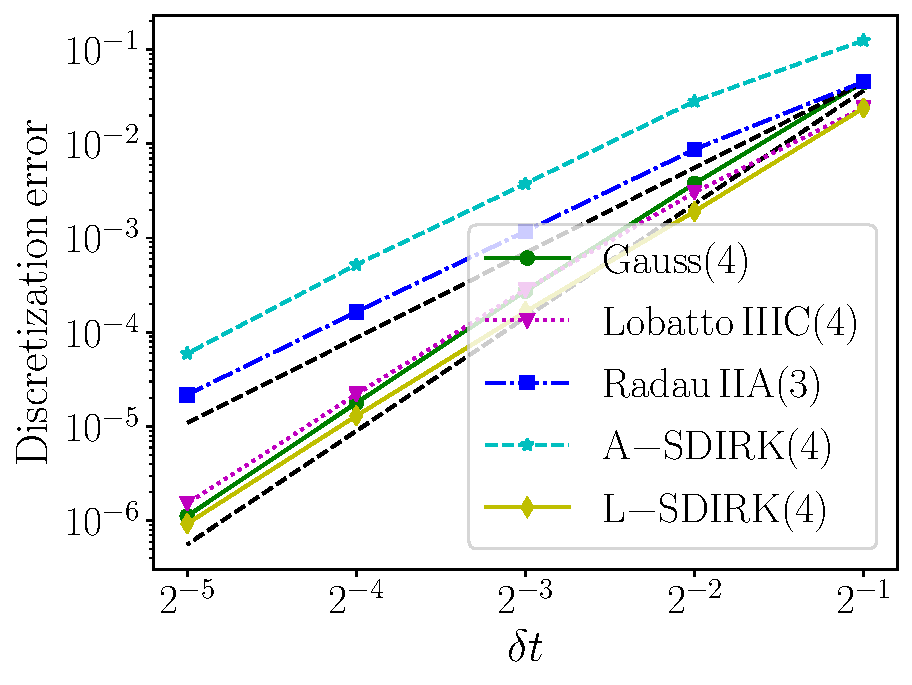
\includegraphics[width = 0.475\textwidth]{figures/FD_ex/errors_iters_14_34_23_-14_4_d2_ex1.pdf}
\quad
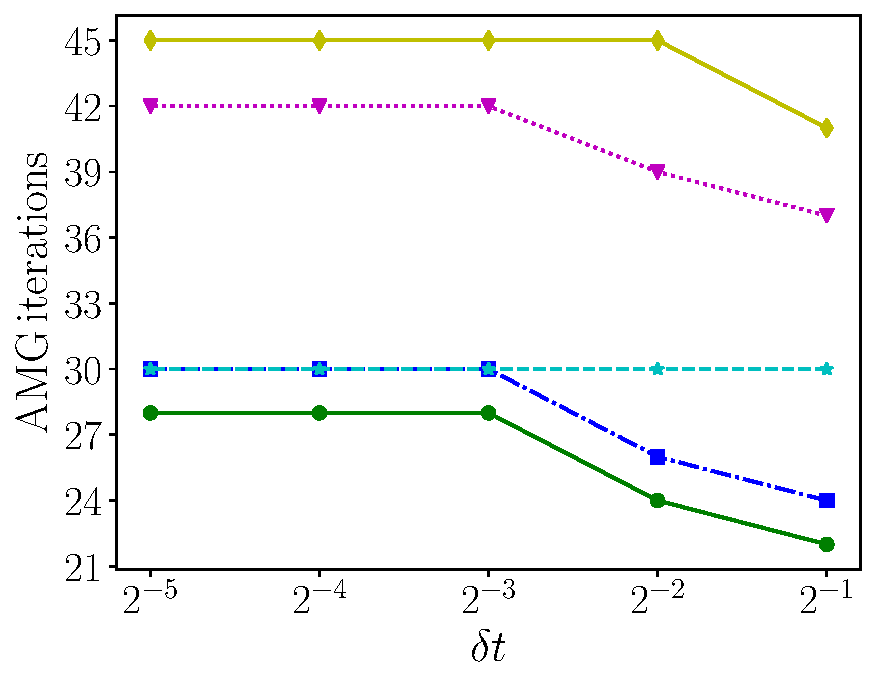
\includegraphics[width = 0.475\textwidth]{figures/FD_ex/amg_iters_14_34_23_-14_4_d2_ex1.pdf}
}
\centerline{
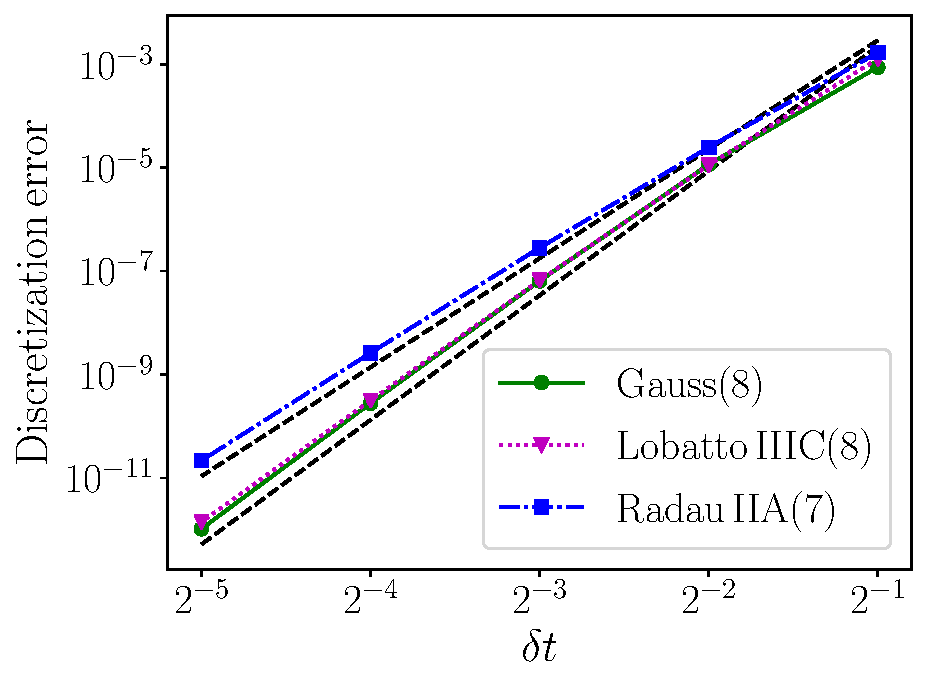
\includegraphics[width = 0.475\textwidth]{figures/FD_ex/errors_iters_18_38_27_d2_ex1.pdf}
\quad
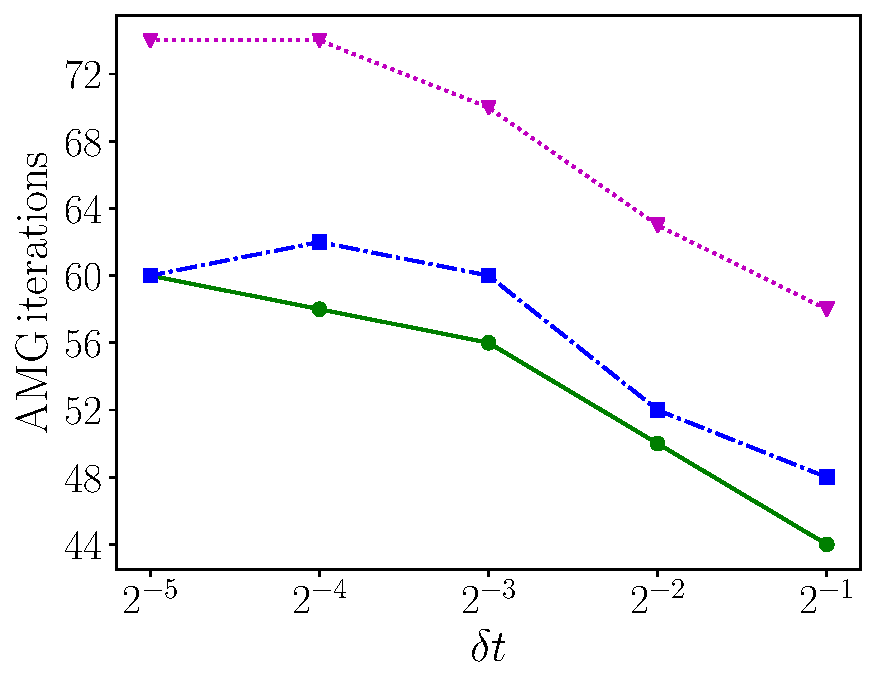
\includegraphics[width = 0.475\textwidth]{figures/FD_ex/amg_iters_18_38_27_d2_ex1.pdf}
}
\caption{Finite-difference advection-diffusion problem \eqref{eq:FD_ex}. $L_{\infty}$-discretization errors at $t = 2$ as a function of time-step $\delta t$ are shown on
the left for various discretizations of approximately 4th order (top) and 8th order (bottom). Black, dashed lines with slopes of three and four are shown (top), as are those with slopes of seven and eight (bottom). Plots on the right show the average number of AMG iterations per time step.
\label{fig:FD_ex}
}
\end{figure}

The preconditioner appears robust with respect to mesh and problem size, since
the average number of AMG iterations per time step (which is a proxy for the
number of GMRES iterations) remains roughly constant as the the mesh is refined.
Of the fully implicit methods, the Gauss methods require the fewest AMG iterations, closely
followed by Radau IIA methods, with the Lobatto IIIC methods requiring the most
AMG iterations. This is
consistent with the theoretical estimates in \Cref{tab:cond}.
Note that while Gauss and Radau IIA methods have very similar
iteration counts, Gauss converges at one order faster, which can be seen in the
left-hand panel of the figure.

Considering the lower-order methods in the top
row of \Cref{fig:FD_ex}, L--SDIRK(4), a 5-stage, 4th-order, L-stable SDIRK
method requires the most AMG iterations of all methods. A--SDIRK(4), a 3-stage,
4th-order, A-stable SDIRK method, requires far fewer AMG iterations than
L--SDIRK(4). However, A--SDIRK(4) yields a significantly larger discretization
error than the other 4th-order schemes, and takes longer to reach its asymptotic
convergence rate. Thus, in terms of work done per accuracy, the new
preconditioner with 4th-order Gauss integration is the clear winner
for this particular test problem, requiring roughly half the AMG iterations
of the commonly used L-stable SDIRK4 scheme.

% ------------------------------------------------------------------------------------- %
% ------------------------------------------------------------------------------------- %
\subsection{DG advection-diffusion}\label{sec:numerics:dg}

Here we consider a more difficult advection-diffusion problem, discretized
using high-order DG finite elements. In particular, we demonstrate
the effectiveness and scalability of the new preconditioning on more complex flows and
DG discretizations (\Cref{fig:ad_advdiff} and \Cref{sec:numerics:dg:adv}),
the reduction in computational work that can be achieved using large time steps and
very high-order integration (\Cref{sec:numerics:dg:adv}), and how
using multiple ``inner'' preconditioning iterations to approximate $\widehat{\mathcal{L}}^{-1}$
(or even inner Krylov acceleration) can be important for the fast, scalable
application of IRK integration (\Cref{sec:numerics:dg:diff}).

The governing equations in spatial domain $\Omega = [0,1] \times [0,1]$ are given by
\begin{equation} \label{eq:adv-diff}
	u_t + \nabla \cdot ( \bm\beta u  - \varepsilon \nabla u ) = f
\end{equation}
where $\bm\beta(x,y) : = (\cos(4\pi y), \sin(2 \pi x))^T$
is the prescribed velocity field and $\varepsilon$ the diffusion coefficient.
Periodic boundary conditions are enforced on $\partial\Omega$, and
\eqref{eq:adv-diff} is discretized with an upwind DG method \cite{Cockburn2001},
where diffusion terms are treated with the symmetric interior penalty method
\cite{Arnold1982,Arnold2002}. The resulting finite element problem is to find
$u_h \in V_h$ such that, for all $v_h \in V_h$,
\[
	\begin{multlined}
	\int_\Omega \partial_t (u_h) v_h \, dx
	- \int_\Omega u_h \bm\beta \cdot \nabla_h v_h \, dx
	+ \int_\Gamma \widehat{u_h} \bm\beta \cdot \llbracket v_h \rrbracket \, ds
	+ \int_\Omega \nabla_h u_h \cdot \nabla_h v_h \, d x \\
	- \int_\Gamma \{ \nabla_h u_h \} \cdot \llbracket v_h \rrbracket \, ds
	- \int_\Gamma \{ \nabla_h v_h \} \cdot \llbracket u_h \rrbracket \, ds
	+ \int_\Gamma \sigma \llbracket u_h \rrbracket \cdot \llbracket v_h \rrbracket \, ds
	= \int_\Omega f v_h \, dx,
	\end{multlined}
\]
where $V_h$ is the DG finite element space consisting of piecewise polynomials of degree
$p$ defined on elements of the computational mesh $\mathcal{T}$ of the spatial domain
$\Omega$. No continuity is enforced between mesh elements.
Here, $\nabla_h$ is the broken gradient, $\Gamma$ denotes the skeleton of the mesh,
and $\{ \cdot \}$ and $\llbracket \cdot \rrbracket$ denote the average and jump of a
function across a mesh interface.
$\widehat{u_h}$ is used to denote the upwind numerical flux.
This discretization has been implemented in the MFEM finite element framework
\cite{Anderson2020}, and uses AMG preconditioning with approximate ideal restriction
(AIR) \cite{Manteuffel:2019,Manteuffel:2018} (after first scaling by the inverse of the
block-diagonal mass matrix).

The DG method is particularly well-suited for advection-dominated problems.
In the following subsections we vary $\varepsilon$ from $0$ (purely advective) to $0.01$.
The velocity field, initial condition, and numerical solution for $\varepsilon = 10^{-6}$
are shown in \Cref{fig:ad_advdiff}.

% srun -n32 ./dg_adv_diff  -rs 3 -rp 1 -i 18 -o 4 -dt 0.1 -air 2 -tf 10 -e 1e-6 -nov
% dt = 0.1, hmin = 0.015625, hmax = 0.015625
% time order = 8, space order = 4
% time acc. = 1e-08, space acc. = 5.96046e-08
%
\begin{figure}[!htb]
  \centering
  \begin{subfigure}[b]{0.3\textwidth}
    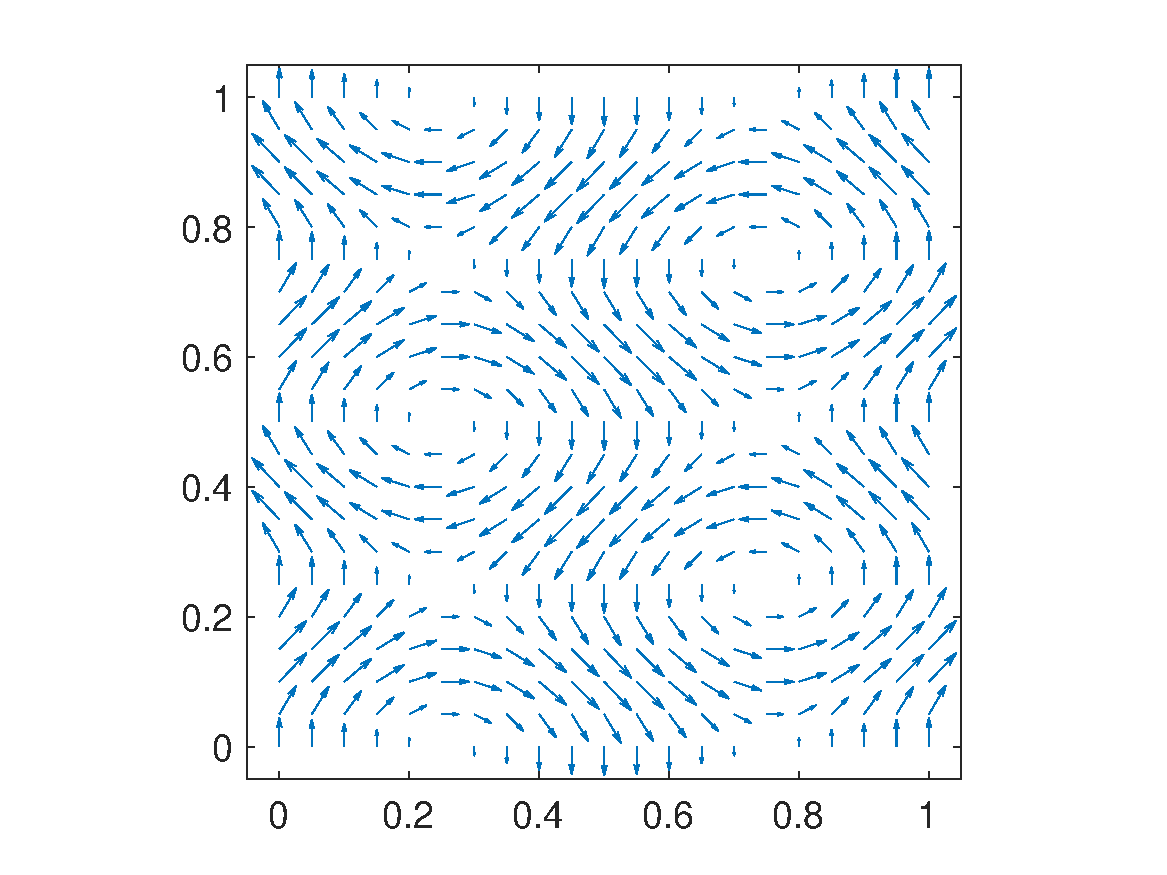
\includegraphics[width=\textwidth]{./figures/velocity_field.pdf}
    \caption{Velocity field}\label{fig:v}
  \end{subfigure}
   \begin{subfigure}[b]{0.3\textwidth}
    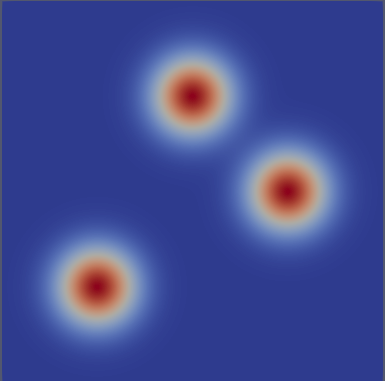
\includegraphics[width=\textwidth]{./figures/solution.0000.png}
    \caption{$t = 0$}
  \end{subfigure}
  \begin{subfigure}[b]{0.3\textwidth}
    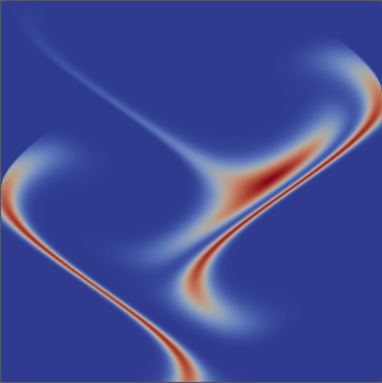
\includegraphics[width=\textwidth]{./figures/solution.0003.png}
    \caption{$t = 0.3$}
  \end{subfigure}
  \\\vspace{2ex}
   \begin{subfigure}[b]{0.3\textwidth}
    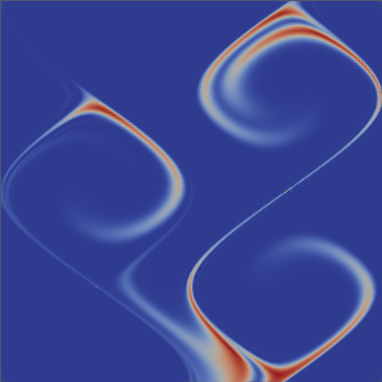
\includegraphics[width=\textwidth]{./figures/solution.0008.png}
    \caption{$t = 0.8$}
  \end{subfigure}
   \begin{subfigure}[b]{0.3\textwidth}
    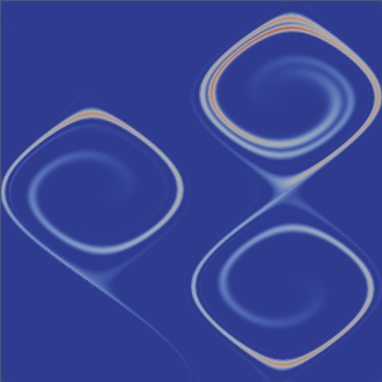
\includegraphics[width=\textwidth]{./figures/solution.0020.png}
    \caption{$t = 2.0$}
  \end{subfigure}
  \begin{subfigure}[b]{0.3\textwidth}
    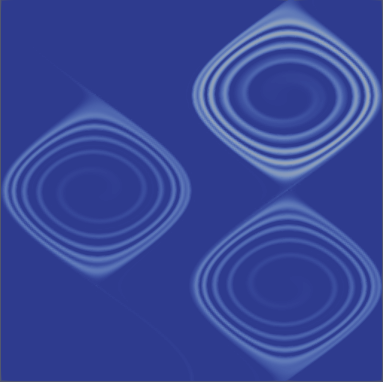
\includegraphics[width=\textwidth]{./figures/solution.0070.png}
    \caption{$t = 7.0$}
  \end{subfigure}
  \\\vspace{2ex}
      \caption{DG advection-diffusion problem with velocity field shown in
      subplot (a) and the solution plotted for various time points from
      $t=0$ to $t = 7.0$ in subplots (b-f). Heatmap indicates solution in the
      2d domain, with blue $\mapsto 0$ and red $\mapsto 1$.}
  \label{fig:ad_advdiff}
\end{figure}

% ------------------------------------------------------------------------------------- %
\subsubsection{A hyperbolic example, and preconditioning with $\eta$ vs. $\gamma_*$}
\label{sec:numerics:dg:const}

First, we demonstrate the effectiveness of using $\gamma_*$ (\Cref{sec:solve:gamma})
instead of $\eta$ in the preconditioner, as well as the robustness of the proposed
method on a fully hyperbolic problem, where most papers have only discussed parabolic
PDEs. Thus, we set the diffusion coefficient $\varepsilon = 0$
and apply AIR as a preconditioner for individual systems
$(\gamma M - \delta t\mathcal{L})$.

AIR was originally designed for upwind DG discretizations of advection
and is well-suited for this problem. We use the \textit{hypre} implementation,
with distance 1.5 restriction with strength tolerance $\theta_R=0.01$, one-point
interpolation (type 100), Falgout coarsening (type 6) with strength tolerance
$\theta_C=0.1$, no pre-relaxation, and forward Gauss Seidel
post-relaxation (type 3), first on F-points followed by a second sweep on
all points. The domain is discretized using 4th-order finite elements on a
structured mesh, and the time step for each integration scheme is chosen
such that the spatial and temporal orders of accuracy match; for example,
for 8th-order integration we choose $\delta t = \sqrt{h}$, for mesh spacing
$h$, so that $\delta t^8 = h^4$. All linear systems are solved to a relative
tolerance of $10^{-12}$. There are a total of 1,638,400 spatial degrees-of-freedom
(DOFs), and the simulations are run on 288 processors on the Quartz machine at
Lawrence Livermore National Lab, resulting in $\sim$5600 DOFs/processor.

\Cref{tab:gamma} shows the average number of AIR iterations to solve for
each pair of stages of an IRK method using $\eta$ and $\gamma_*$ as the preconditioning
constants. Iteration counts are shown for Gauss, Radau IIA, and Lobatto IIIC integration,
with 2--5 stages, and the (factor of) reduction in iteration count achieved using $\gamma_*$
vs. $\eta$ is also shown. For 5-stage Lobatto IIIC integration, $\gamma_*$ yields
almost a $6\times$ reduction in total inner AIR iterations to solve for the
``hard'' stage ($\beta > \eta$), while in no cases is there an increase in
iteration count when using $\gamma_*$.

{
% \renewcommand{\tabcolsep}{4pt}
\renewcommand{\arraystretch}{1.15}
\begin{table}[!ht]
  \centering
  \begin{tabular}{|l || r | rr | rr | rrr |}  % chktex 44
  \hline
\multicolumn{9}{|c|}{Gauss}\\\hline
Stages/Order & 2/4 & \multicolumn{2}{c}{3/6} & \multicolumn{2}{|c}{4/8} & \multicolumn{3}{|c|}{5/10} \\\hline
Iterations$(\eta)$ & 17 & 6 & 30 & 11  & 47 & 8 & 16 & 70 \\
Iterations$(\gamma_*)$ & 11 & 6 & 15 & 10 & 19 & 8 & 13 & 23 \\\hline
Speedup & 1.5 & 1.0 & 2.0 & 1.1 & 2.5 & 1.0 & 1.2 & 3.0 \\\hline\hline
\multicolumn{9}{|c|}{Radau IIA}\\\hline
Stages/Order & 2/3 & \multicolumn{2}{c}{3/5} & \multicolumn{2}{|c}{4/7} & \multicolumn{3}{|c|}{5/9} \\\hline
Iterations$(\eta)$ & 12 & 5 & 39 & 11 & 64 & 8 & 16 & 97 \\
Iterations$(\gamma_*)$ & 12 & 5 & 18 & 9 & 21 & 8 & 12 & 25 \\\hline
Speedup & 1.0 & 1.0 & 2.2 & 1.2 & 3.0 & 1.0 & 1.3 & 3.9 \\\hline\hline
\multicolumn{9}{|c|}{Lobatto IIIC}\\\hline
Stages/Order & 2/2 & \multicolumn{2}{c}{3/4} & \multicolumn{2}{|c}{4/6} & \multicolumn{3}{|c|}{5/8} \\\hline
Iterations$(\eta)$ & 8 & 3 & 67 & 11 & 113 & 7 & 17 & 175 \\
Iterations$(\gamma_*)$ & 8 & 3 & 22 & 9 & 26 & 7 & 12 & 30 \\\hline
Speedup & 1.0 & 1.0 & 3.0 & 1.2 & 4.3 & 1.0 & 1.4 & 5.8 \\\hline\hline
  \end{tabular}
  \caption{Average AIR iterations to solve for each stage in an implicit
  Runge-Kutta method using preconditioners $(\eta M - \delta t \mathcal{L})^{-2}$ and
  $(\gamma_* M - \delta t \mathcal{L})^{-2}$, with $\gamma_*$ defined in \eqref{eq:gamma*}. 
  The ratio of iterations$(\eta)$/iterations$(\gamma_*)$ is shown in the ``Speedup'' rows.}
  \label{tab:gamma}
\end{table}
}


% ------------------------------------------------------------------------------------- %
\subsubsection{Advection-dominated}\label{sec:numerics:dg:adv}

This section demonstrates high-order IRK integration applied to the advection-dominated
problem in \Cref{fig:ad_advdiff}, using AIR as a preconditioner for the linear
systems.

\Cref{fig:dg_o4_abs} shows the total number of AIR iterations required to
compute one time step using six different Runge-Kutta schemes, from 4th
to 10th order, as a function of mesh spacing $h$. Note that as $h\to 0$,
there is only modest growth in the number of AIR iterations per time step,
indicating good (but not perfect) scalability.
Moreover, note that there is small growth in the number of iterations for
SDIRK4 as well (increasing from 20 to 25), which suggests the growth in
iteration count is due to imperfect scalability of AIR iterations rather
than the new IRK preconditioning.

\Cref{fig:dg_o4_rel} then shows the relative number of AIR iterations to
compute a given accuracy compared to SDIRK4. For example, if $h=0.01$,
then SDIRK4 uses $\delta t_4 = 0.01$ and Gauss8 uses $\delta t_8 =
\sqrt{0.01} = 0.1 = 10\delta t_4$, that is, $10\times$ less time steps to
achieve comparable accuracy. Note that as $h\to 0$, this factor becomes progressively
larger. For quite moderate $h$, we see how very high-order integration
can quickly lead to a reduction in total preconditioning iterations compared to a
standard SDIRK4 scheme. Gauss8 and Radau9, for example, require almost
$7\times$ less AIR iterations than SDIRK4 at $h =\delta t_4 = 1/256$,
and this ratio continues to decrease for smaller $\delta t$. Although this
does not account for additional setup time, where Gauss8 and Radau9 require
solving two and three different linear systems, respectively, and SDIRK4
only one, very high-order
integration permitted through the new preconditioning still offers the
opportunity for significant speedups.

%
\begin{figure}[!h]
  \centering
  \begin{subfigure}[b]{0.475\textwidth}
    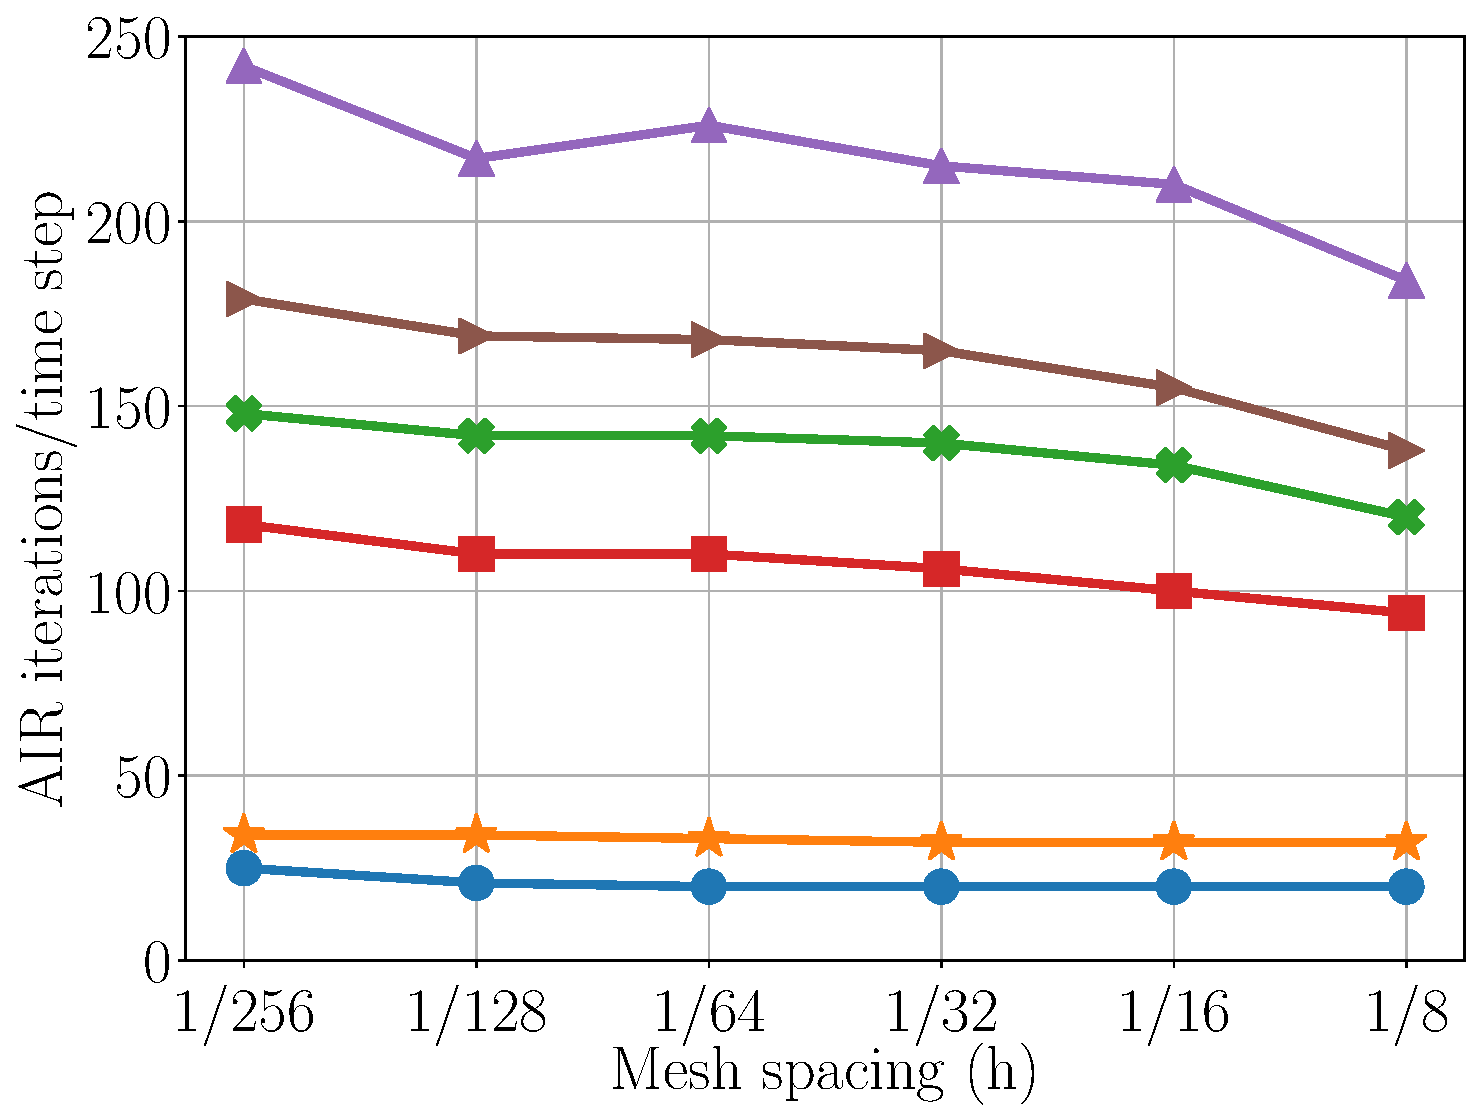
\includegraphics[width=\textwidth]{./figures/dg_advdiff_o4_1e-6.pdf}
    \caption{Total AIR iterations per time step}
	\label{fig:dg_o4_abs}
  \end{subfigure}
   \begin{subfigure}[b]{0.475\textwidth}
    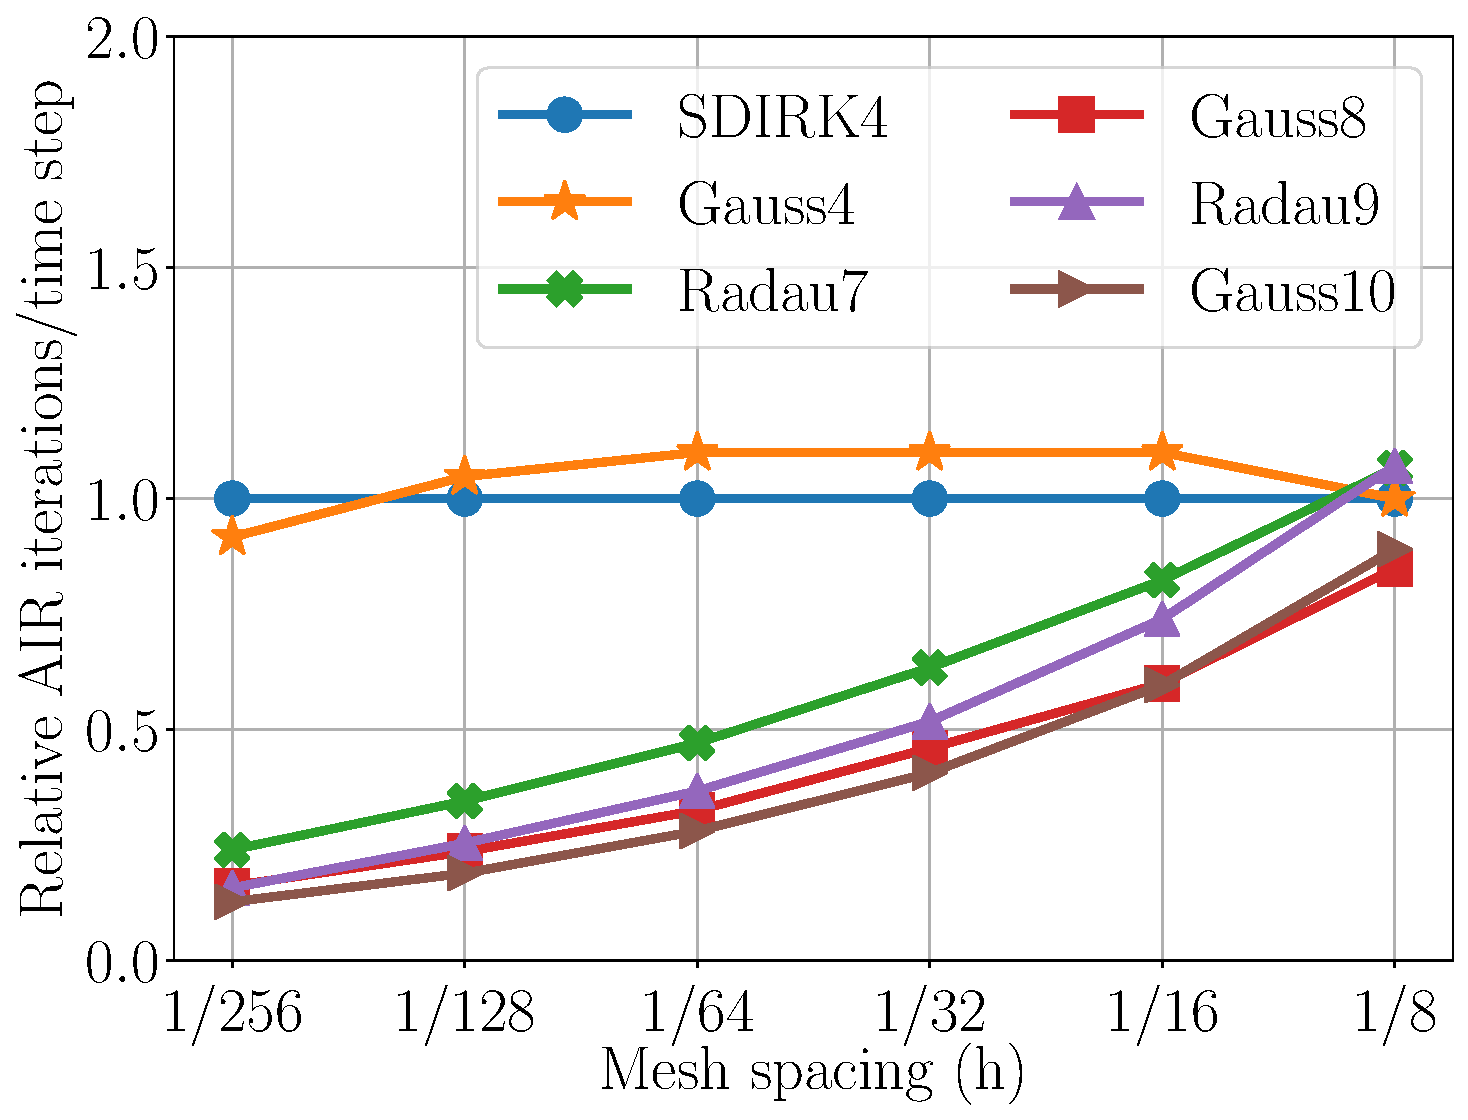
\includegraphics[width=\textwidth]{./figures/dg_advdiff_o4_1e-6_rel.pdf}
   \caption{AIR iterations relative to SDIRK4}
	\label{fig:dg_o4_rel}
  \end{subfigure}
\caption{}
  \label{fig:dg_o4}
\end{figure}
%


% ------------------------------------------------------------------------------------- %
\subsubsection{Diffusive problems and inner Krylov}\label{sec:numerics:dg:diff}

In \cite{Manteuffel:2019}, AIR was shown to be effective on some DG advection-diffusion
problems, and classical AMG is known to be effective on diffusion-dominated
problems. However, the region of comparable levels of advection and diffusion
remains the most difficult from a multigrid perspective. We use this to
demonstrate how methods developed here require a ``good'' preconditioner
for a backward Euler time step, $(\gamma M - \delta t \mathcal{L})^{-1}$,
in order to converge on more general IRK
methods. Fortunately, ensuring a preconditioner is sufficiently good can be
resolved by appealing to standard block preconditioning techniques, where an inner
iteration is used that applies multiple AIR iterations as a single preconditioner.

Here we consider an analogous problem to above, but set the diffusion coefficient
to $\varepsilon = 0.01$. We use a mesh with spacing $h \approx 0.001$, 2nd-order
DG finite elements, a time step of $\delta t = 0.1$, and three-stage 6th-order
Gauss integration. Altogether, this yields equal orders of accuracy, with time and
space error $\sim10^{-6}$. FGMRES \cite{saad1993flexible} is used for the
outer iteration, which allows for GMRES to be applied in an inner iteration
as a preconditioner for $(\gamma_* M - \delta t \mathcal{L})$. \Cref{fig:dg_o2} plots the
total number of AIR iterations per time step as a function of the number of
AIR iterations applied for each application of the preconditioner, using an
inner GMRES or an inner fixed-point (Richardson) iteration. An advection-dominated
problem with $\varepsilon = 10^{-6}$ is also shown for comparison.

Recall we have three stages, one of which is a single linear system corresponding
to a real eigenvalue, and the other corresponding to a pair of complex conjugate
eigenvalues, which we precondition as in \Cref{sec:solve}. The latter ends up being
the more difficult problem to solve -- for $\varepsilon =0.01$ (\Cref{fig:dg_o2_1e-2}),
the outer FGMRES iteration for the complex conjugate quadratic does not converge in
1000 iterations when using one AIR iteration as a preconditioner.
If two AIR iterations with GMRES are used as a preconditioner,
the FGMRES iteration converges in approximately 130 iterations, each of which
requires two applications of GMRES preconditioned with two AIR iterations,
yielding just over 500 total AIR iterations to converge. Further increasing
the number of AIR iterations per preconditioning yields nice convergence
using inner fixed-point or GMRES, with 150 and 112 total AIR iterations per
time step, respectively. In contrast, \Cref{fig:dg_o2_1e-6} shows that
additional AIR iterations for the advection-dominated case are generally
detrimental to overall computational cost (although the outer iteration
converges slightly faster, it does not make up for the additional linear
solves/iteration).

\begin{figure}[h!]
\centering

  \centering
  \begin{subfigure}[b]{0.475\textwidth}
	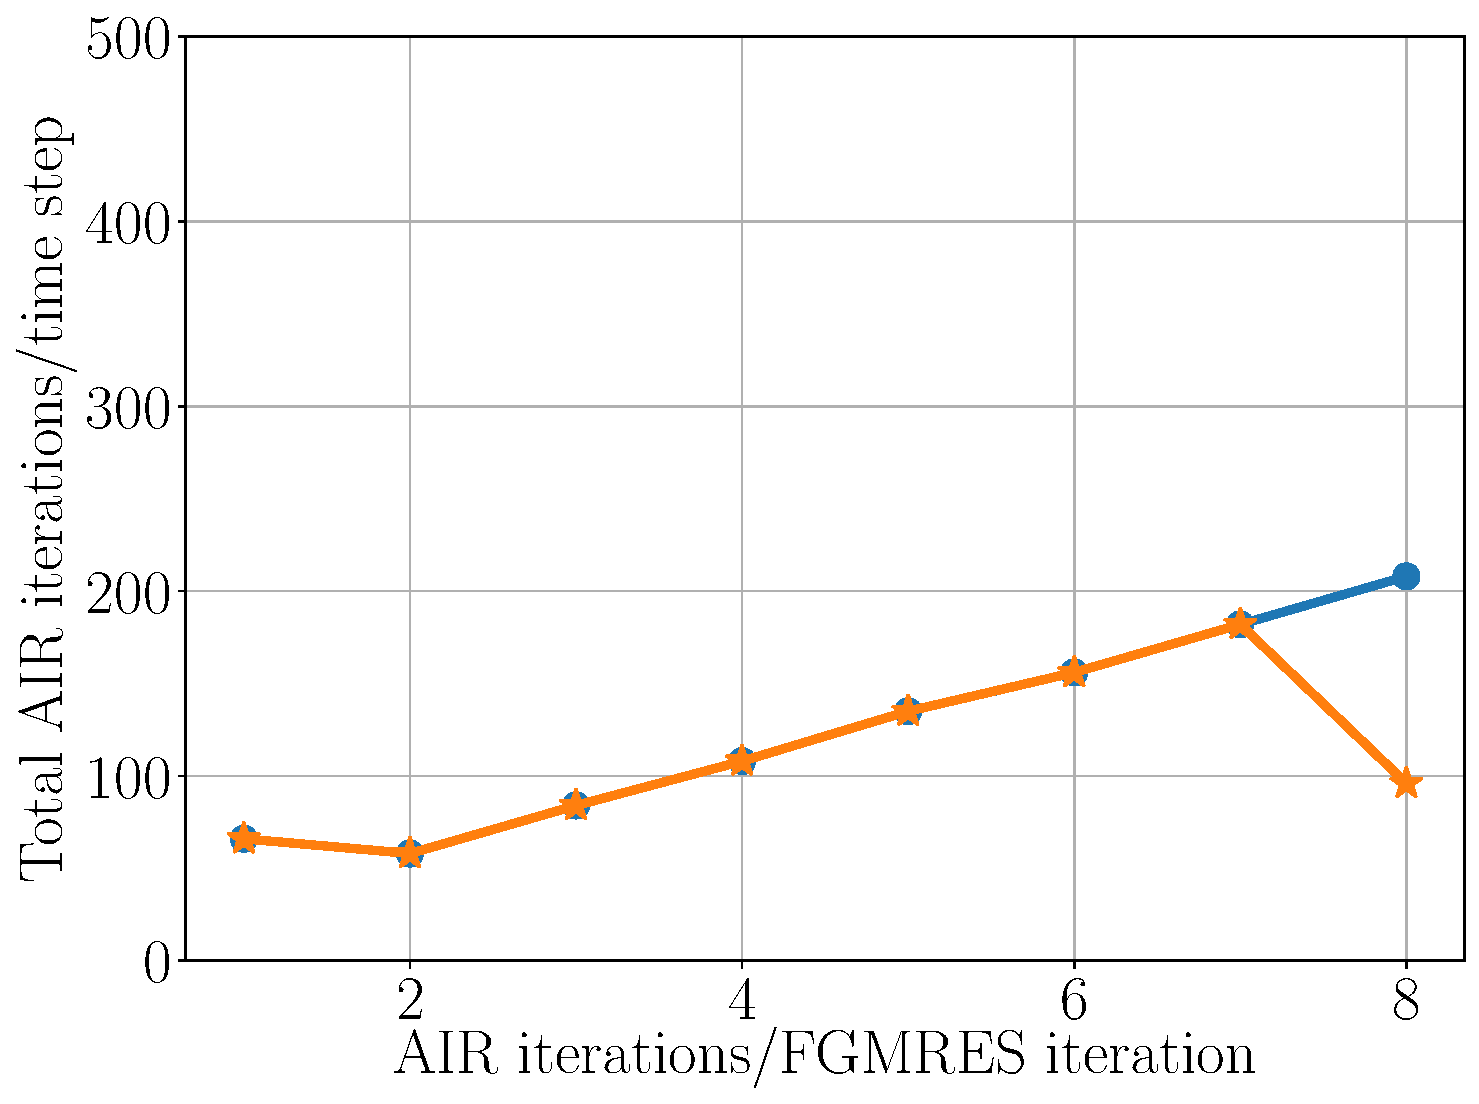
\includegraphics[width = \textwidth]{./figures/dg_advdiff_o2_1e-6.pdf}
	\caption{$\varepsilon = 10^{-6}$.}
	\label{fig:dg_o2_1e-6}
  \end{subfigure}
   \begin{subfigure}[b]{0.475\textwidth}
	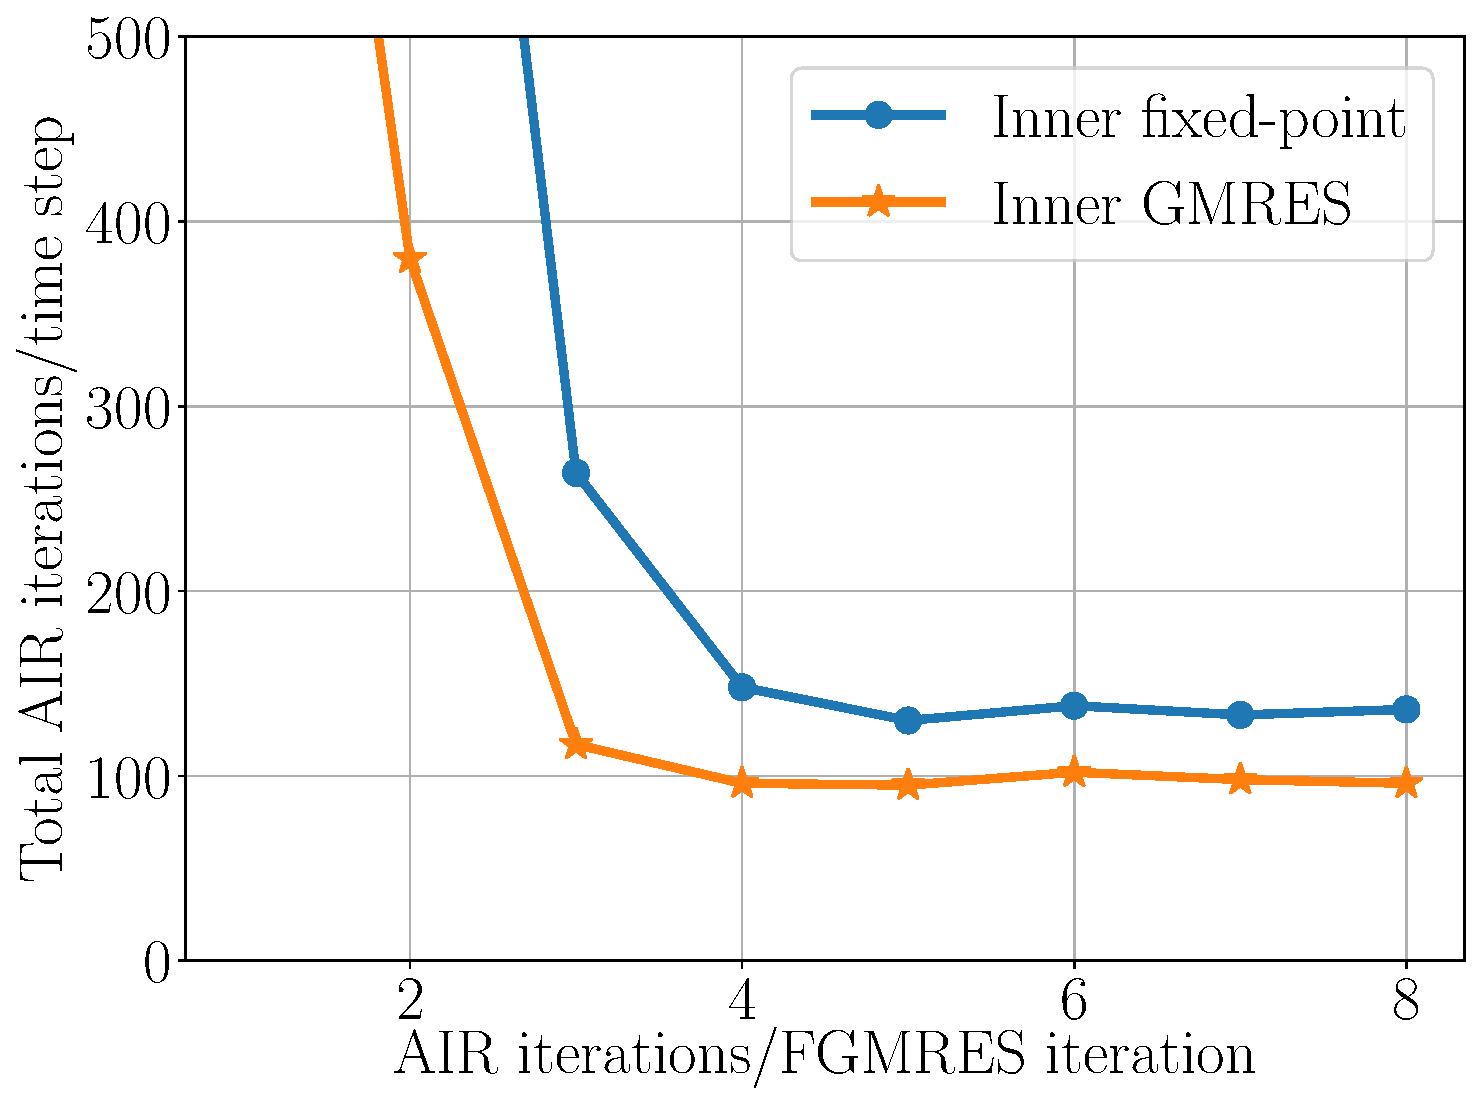
\includegraphics[width = \textwidth]{./figures/dg_advdiff_o2_1e-2.pdf}
	\caption{$\varepsilon = 0.01$.}
	\label{fig:dg_o2_1e-2}
  \end{subfigure}
\caption{AIR iterations per time step as a function of the number of
AIR iterations applied in each application of the preconditioner, for
diffusion coefficient $\varepsilon$.}
\label{fig:dg_o2}
\end{figure}


% ------------------------------------------------------------------------------------- %
% ------------------------------------------------------------------------------------- %
\subsection{High-order matrix-free diffusion}

In this example, we illustrate the use of high-order IRK methods coupled with high-order finite element spatial discretizations.
It is well-known that matrix assembly becomes prohibitively expensive for high-order finite elements.
Naive algorithms typically require $\mathcal{O}(p^{3d})$ operations to assemble the resulting system matrix, where $p$ is the polynomial degree and $d$ is the spatial dimension.
Techniques such as sum factorization can reduce this cost on tensor-product elements to $\mathcal{O}(p^{2d+1})$, however this cost can still be prohibitive for large values of $p$ \cite{Melenk2001}.
On the other hand, matrix-free operator evaluation on tensor-product meshes can be performed in $\mathcal{O}(p^{d+1})$ operations \cite{Orszag1980}, motivating the development of solvers and preconditioners that can be constructed and applied without access to the assembled system matrix \cite{Kronbichler2019}.

We consider a high-order finite element discretization of the linear heat equation on spatial domain $\Omega$,
\[
	\int_\Omega \partial_t (u_h) v_h \, dx + \int_\Omega \nabla u_h \cdot \nabla v_h \, dx = \int_\Omega f v_h \, dx,
\]
where $u_h, v_h \in V_h$, and $V_h$ denotes the degree-$p$ $H^1$-conforming finite element space defined on a mesh $\mathcal{T}$ consisting of tensor-product elements (i.e.\ quadrilaterals or hexahedra).
The matrix-free action of the corresponding operator is computed in $\mathcal{O}(p^{d+1})$ operations using the \textit{partial assembly} features of the MFEM finite element library \cite{Anderson2020}.
In order to precondition the resulting system, we make use of a low-order refined preconditioner, whereby the high-order system is preconditioned using a spectrally equivalent low-order finite element discretization computed on a refined mesh \cite{Canuto2010}.
The low-order refined discretization can be assembled in $\mathcal{O}(p^d)$ time, thereby avoiding the prohibitive costs of high-order matrix assembly.
We make use of the uniform preconditioners for the low-order refined problem based on subspace corrections, developed in \cite{Pazner2019a}.

For this test case, take the spatial domain to be $\Omega = [0,1] \times [0,1]$, with periodic boundary conditions.
We choose the forcing term
\[
	f(x, y, t) = \sin (2\pi x)\cos(2\pi y) \left(\cos(t) + 8 \pi^2 (2 + \sin(t)) \right),
\]
which corresponds to the exact solution
\[
	u(x, y, t) = \sin(2\pi x)\cos(2\pi y)(2 + \sin(t)).
\]
We begin with a very coarse $3 \times 3$ mesh, and integrate in time until $t=0.1$ using the Gauss and Radau IIA methods of orders 2 through 10.
For each test case, the finite element polynomial degree is set to $k-1$, where $k$ is the order of accuracy of the time integration method, resulting in $k$th order convergence in both space and time.
The mesh and time step are refined by factors of two to confirm the high-order convergence in space and time of the method.
The relative $L^2$ error, obtained by comparing against the exact solution, is shown in \Cref{fig:high-order-diff-errors}.

\begin{figure}[!ht]
	\centering
	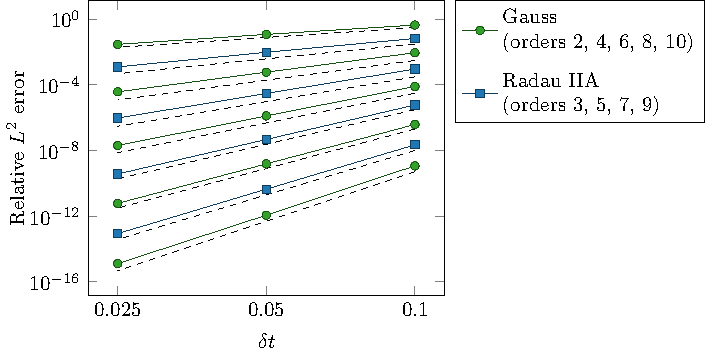
\includegraphics{figures/high_order_diff_error_plot/ho_diff_errors}
	\caption{
		High-order convergence in space and time for the matrix-free diffusion problem.
		Gauss and Radau IIA methods of orders 2 through 10 are used.
		The dashed lines indicate the expected rates of convergence for each method.
	}
	\label{fig:high-order-diff-errors}
\end{figure}

We also use this test case to study the effect of inner iterations on the convergence of the iteration solver.
As discussed in \Cref{sec:inexact-precond}, it is important that the underlying preconditioner provides a good approximation of the inverse of the operator.
For that reason, we consider the use of an inner Krylov solver at every iteration.
Since this corresponds to using a variable preconditioner at each iteration, a flexible Krylov method may have to be used for the outer iteration, although in practice good convergence is often still observed using the standard CG method \cite{Notay2000}.
In particular, we compare the total number of preconditioner applications required to converge the outer iteration to a relative tolerance of $10^{-10}$, both with and without an inner Krylov solver.
For the inner Krylov solver, we use a CG iteration with the same relative tolerance as the outer iteration in order to give a good approximation to the inverse of the operator.
The iteration counts are displayed in \Cref{fig:high-order-diff-iters}.
We note that for the fully implicit IRK methods, using an inner Krylov solver can reduce the total number of preconditioner applications by about a factor of 1.5, although this depends on the type of method and order of accuracy.
As expected, the use of inner iterations does not reduce the total number of preconditioner applications for DIRK methods.
In addition, for this test case, the total number of preconditioner applications required for the second and fourth order Gauss IRK methods is between 1.3 and 2 times smaller than those required for the corresponding equal-order DIRK methods.

\begin{figure}[!ht]
	\centering
	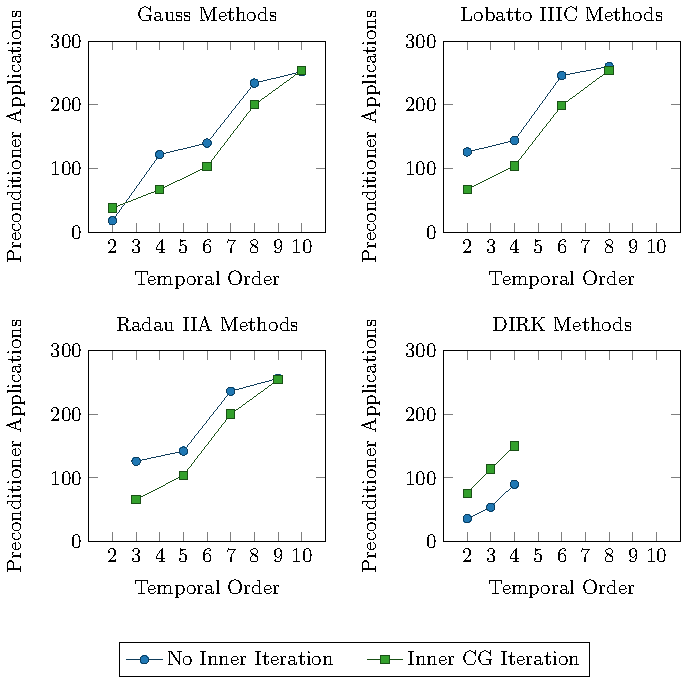
\includegraphics{figures/high_order_diff_iters/high_order_diff_iters}
	\caption{
		Comparison of total number of preconditioner applications with and without
		inner iterations.
		Both the outer iteration and the inner CG iteration are converged to a
		relative tolerance of $10^{-10}$.
	}
	\label{fig:high-order-diff-iters}
\end{figure}

% ------------------------------------------------------------------------------------- %
% ------------------------------------------------------------------------------------- %
% ------------------------------------------------------------------------------------- %
\section{Conclusions}\label{sec:conc}

This paper introduces a theoretical and algorithmic framework for the fast, parallel
solution of fully implicit Runge-Kutta and DG discretizations in time for linear
numerical PDEs. Theory is developed to guarantee $\mathcal{O}(1)$ conditioning under
general assumptions on the spatial discretization that yield stable time integration.
Numerical results demonstrate the new method on various high-order finite-difference
and finite-element discretizations of linear parabolic and hyperbolic problems,
demonstrating fast, scalable solution of up to 10th order accuracy. In several
cases, the new method can achieve 4th-order accuracy using Gauss integration
with roughly half the number of preconditioner applications as required using
standard SDIRK techniques. Ongoing work involves addressing fully nonlinear
problems and algebraic constraints, in particular, without assuming that the
linear system \eqref{eq:k0} can be expressed in Kronecker-product form (thus
allowing for a true Newton or better Newton-like method compared with the
commonly used/analyzed simplified Newton approach).

% ------------------------------------------------------------------------------- %
\bibliographystyle{siamplain}
\bibliography{refs2.bib}


\end{document}
